\begin{appendices}
	\chapter{Convergence}
	\label{app:convergence}
	\begin{figure}[!htb]
		\centering
		\begin{subfigure}{.32\textwidth}
			\centering
			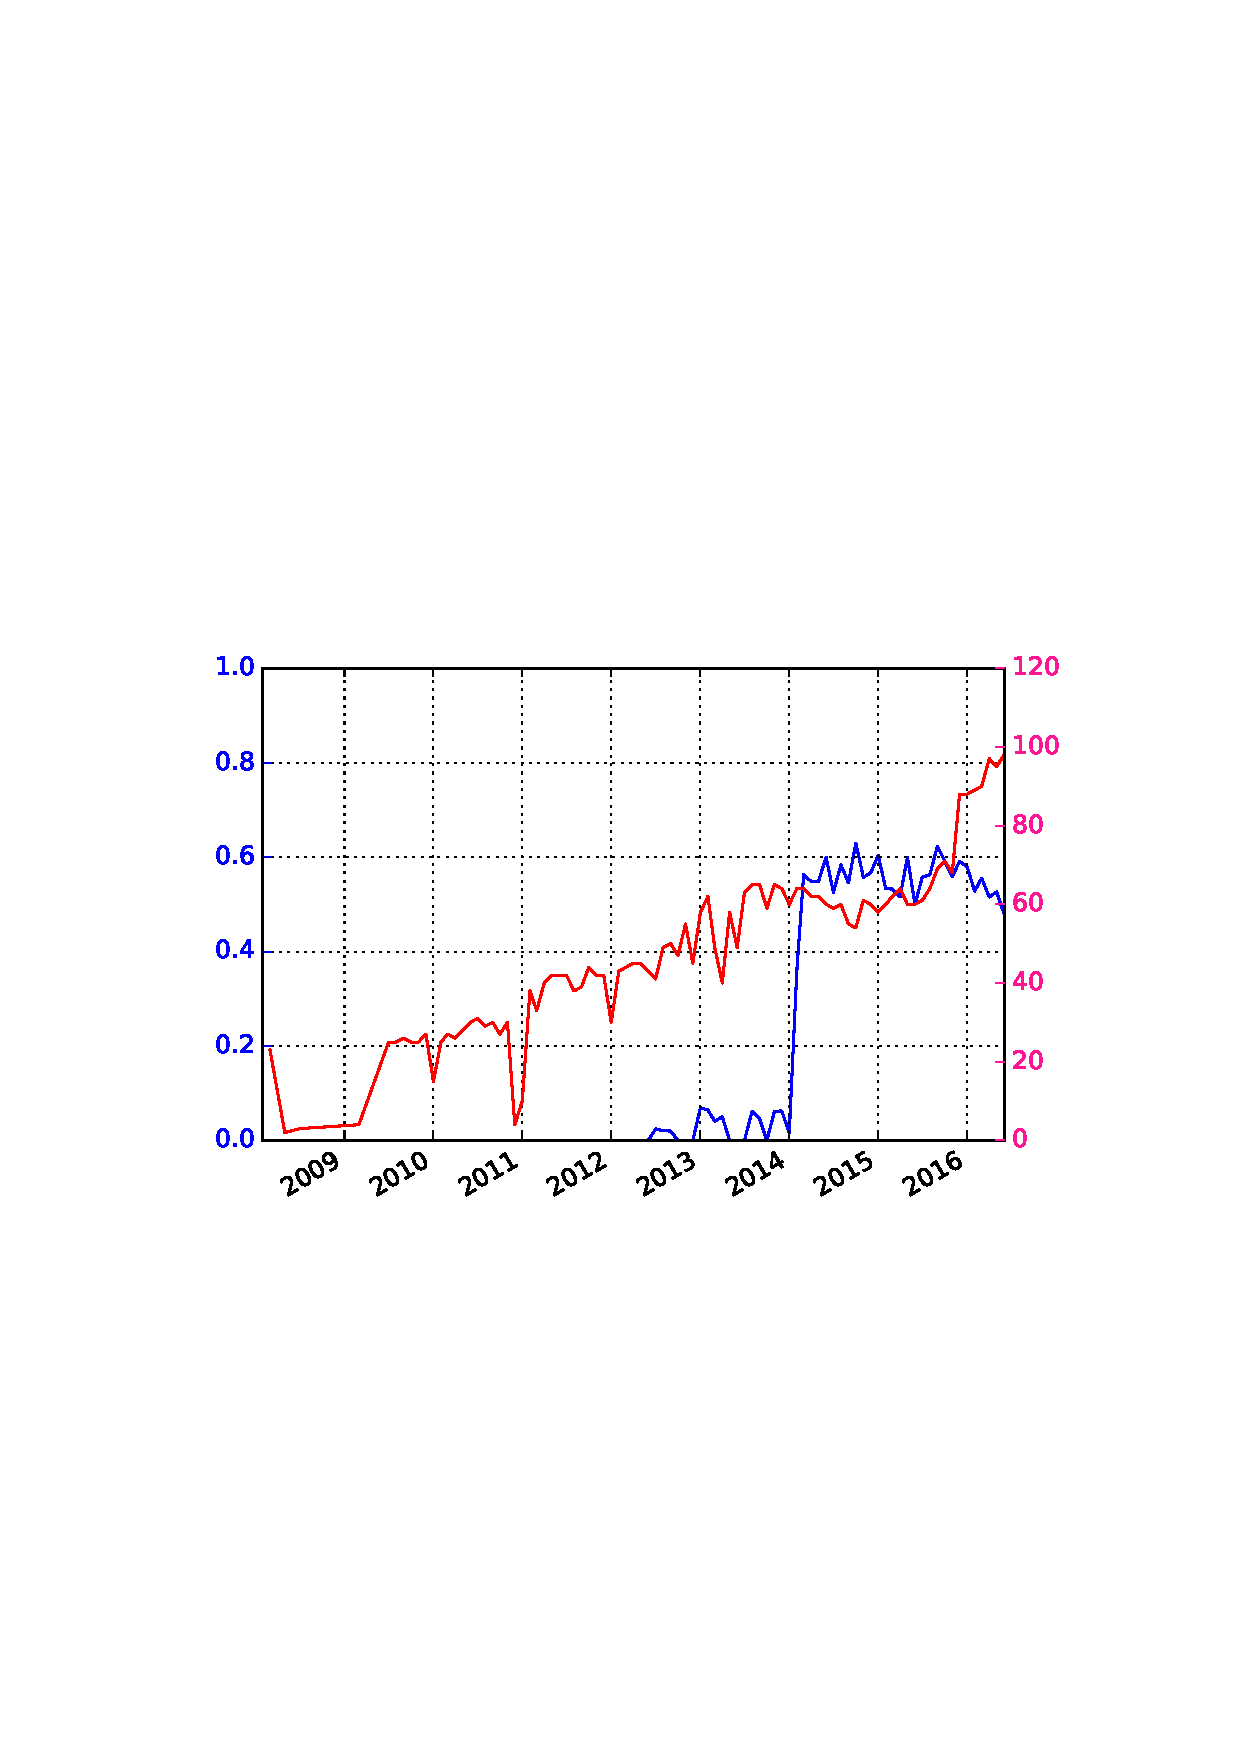
\includegraphics[width=\linewidth]{img/convergence_over_time_a.png}
			\caption{A-Root}
			\label{fig:convergence-a}			
		\end{subfigure}
		\begin{subfigure}{.32\textwidth}
			\centering
			\includegraphics[width=\linewidth]{img/convergence_over_time_c.png}
			\caption{C-Root}
			\label{fig:convergence-c}
		\end{subfigure}		
		\begin{subfigure}{.32\textwidth}
			\centering
			\includegraphics[width=\linewidth]{img/convergence_over_time_d.png}
			\caption{D-Root}
			\label{fig:convergence-d}
		\end{subfigure}		
		\begin{subfigure}{.32\textwidth}
			\centering
			\includegraphics[width=\linewidth]{img/convergence_over_time_f.png}
			\caption{F-Root}
			\label{fig:app:convergence-f}
		\end{subfigure}				
		\begin{subfigure}{.32\textwidth}
			\centering
			\includegraphics[width=\linewidth]{img/convergence_over_time_i.png}
			\caption{I-Root}
			\label{fig:convergence-i}
		\end{subfigure}								
		\begin{subfigure}{.32\textwidth}
			\centering
			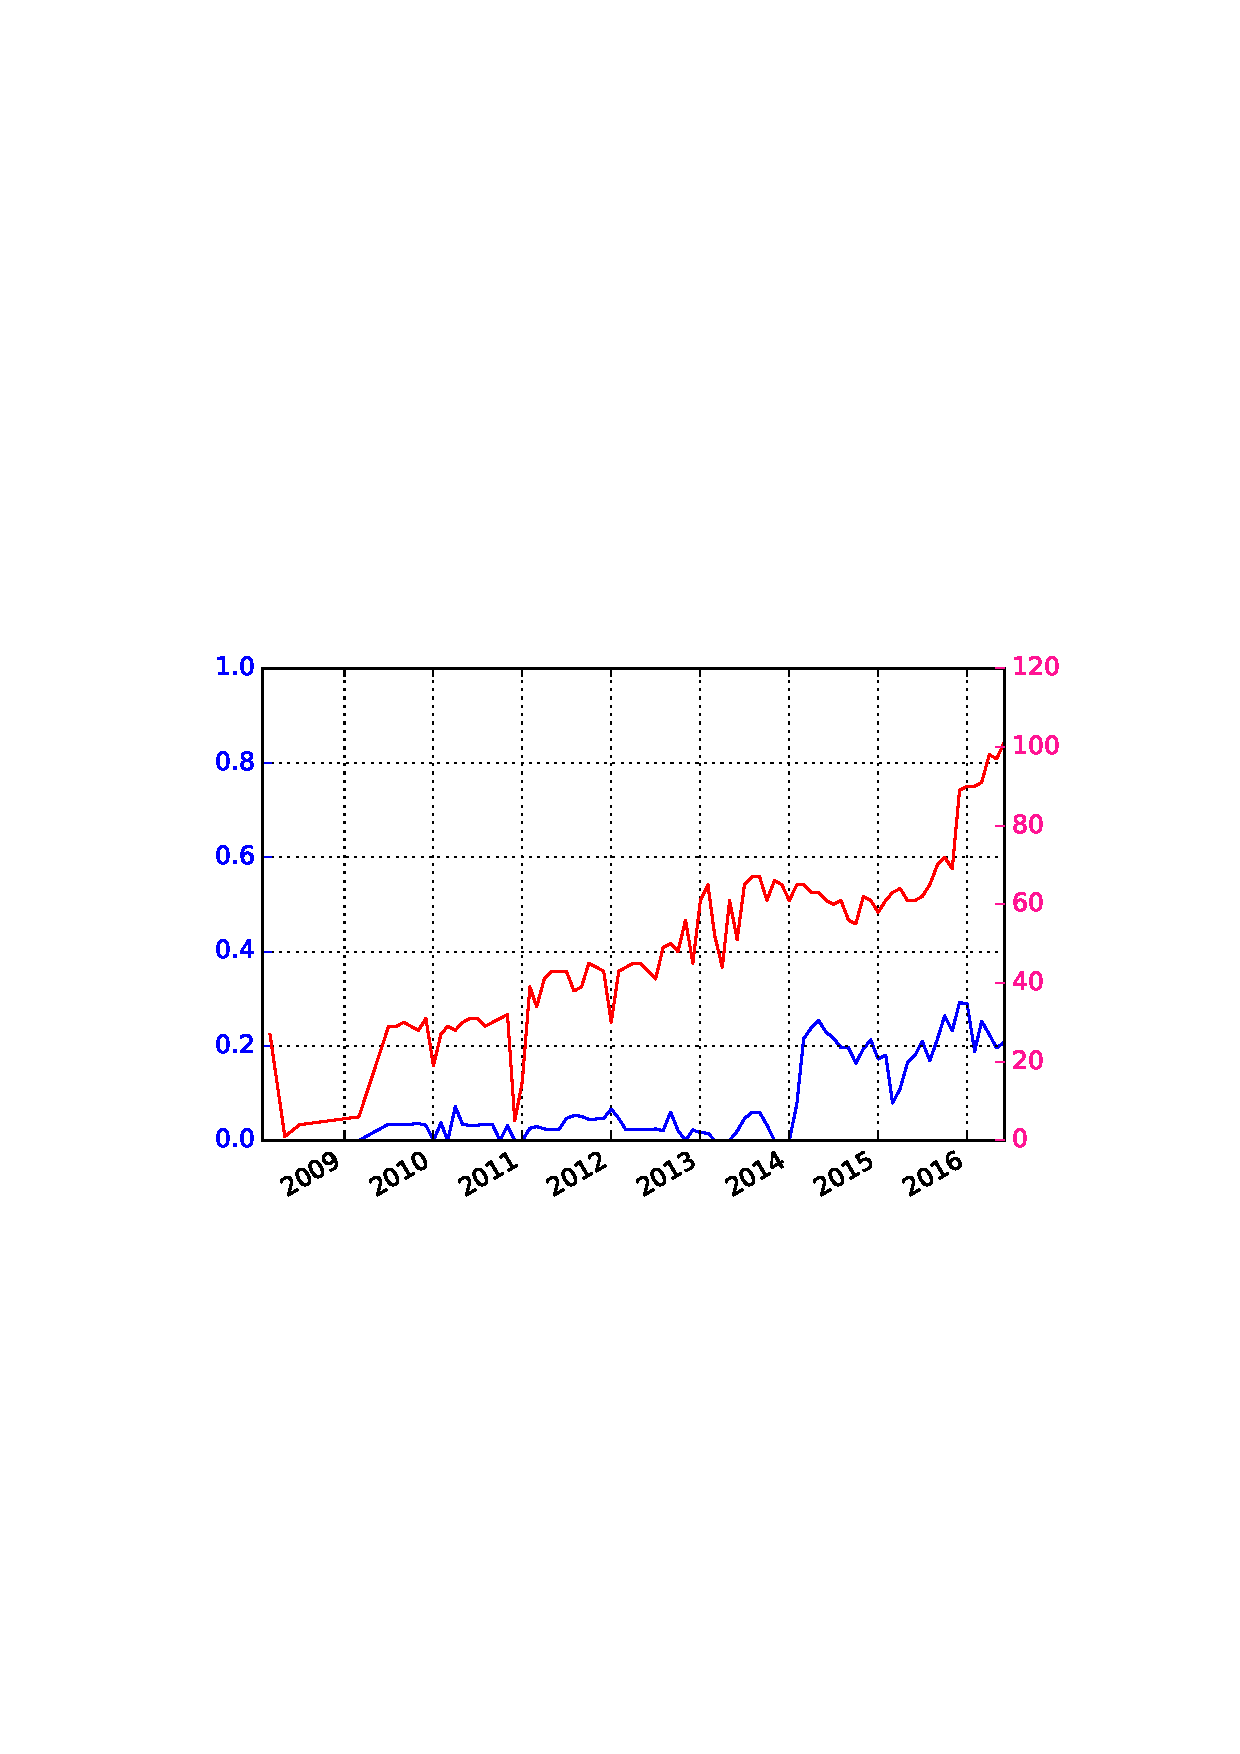
\includegraphics[width=\linewidth]{img/convergence_over_time_j.png}
			\caption{J-Root}
			\label{fig:convergence-j}
		\end{subfigure}										
		\begin{subfigure}{.32\textwidth}
			\centering
			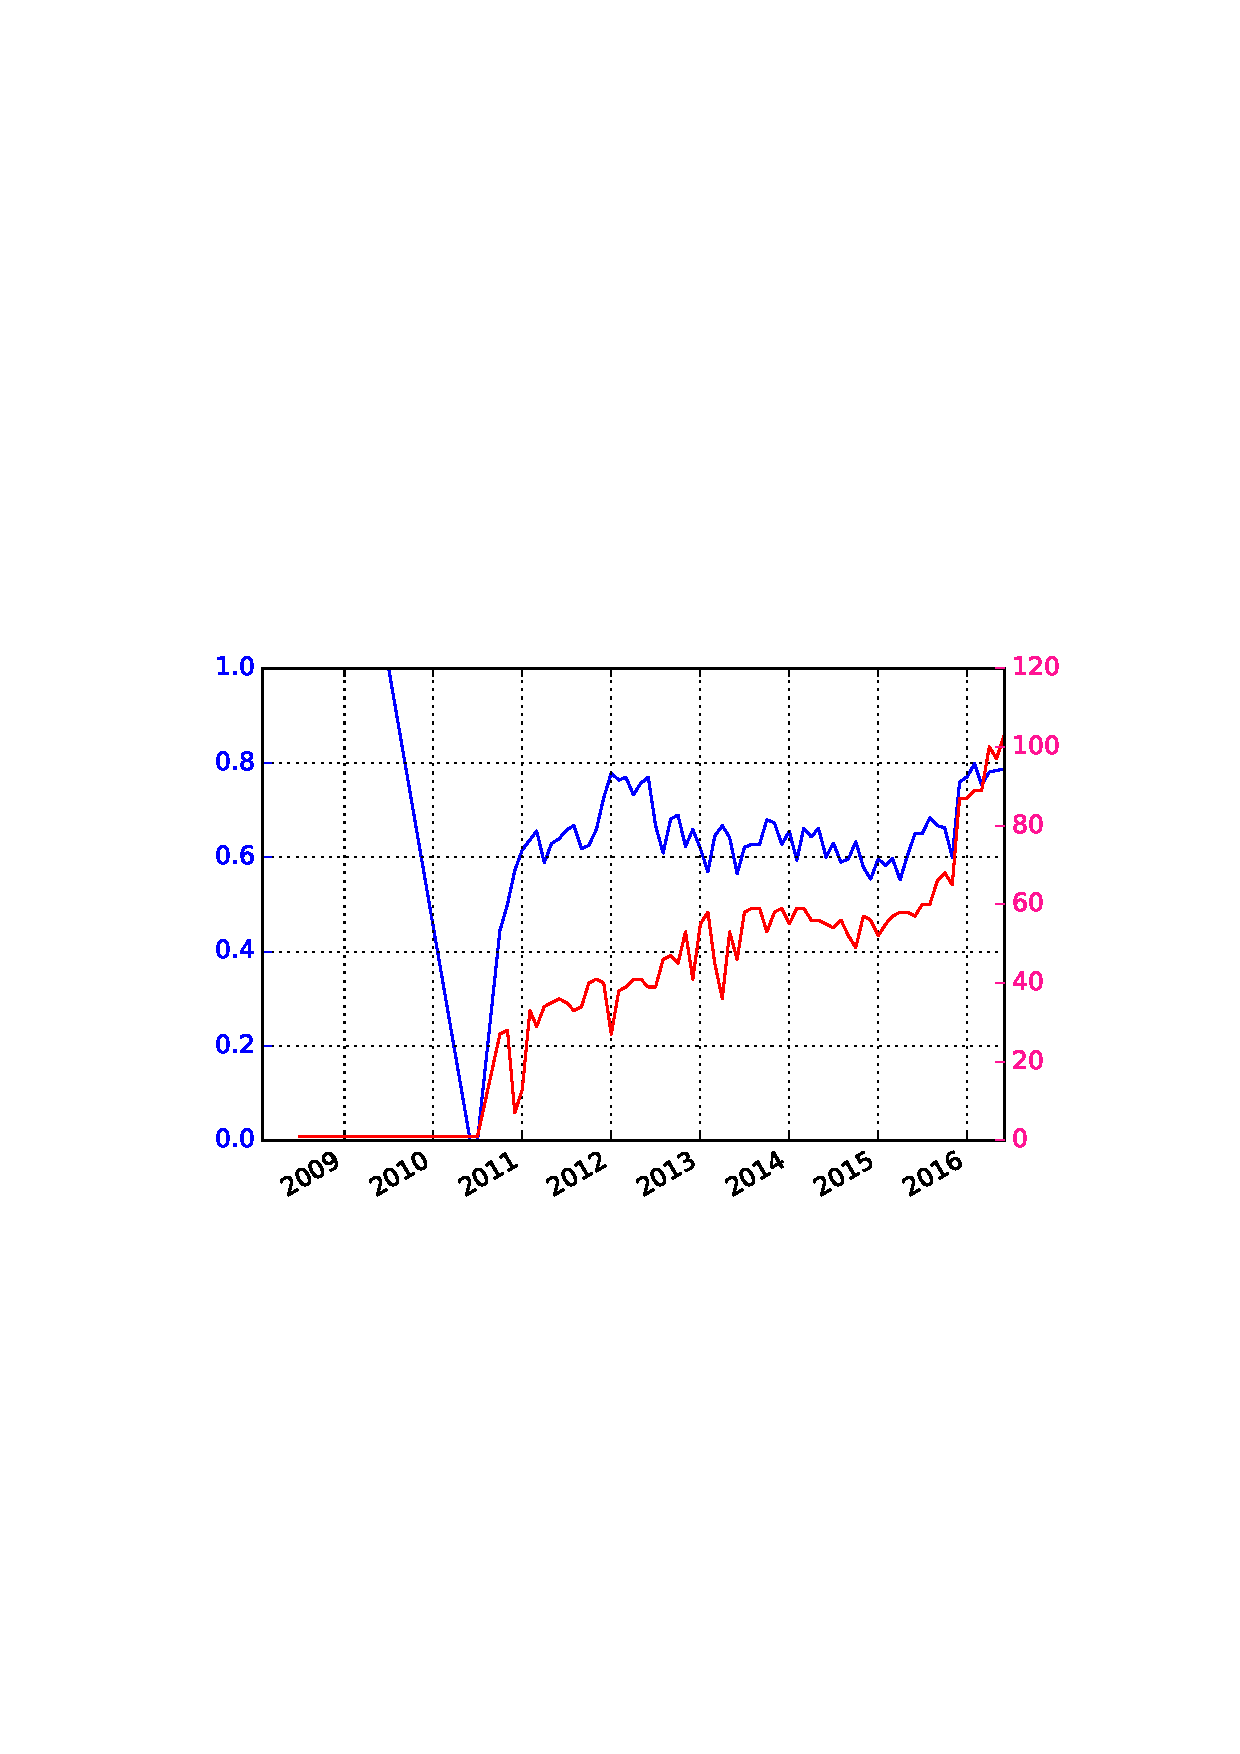
\includegraphics[width=\linewidth]{img/convergence_over_time_k.png}
			\caption{K-Root}
			\label{fig:convergence-k}
		\end{subfigure}											
		\begin{subfigure}{.32\textwidth}
			\centering
			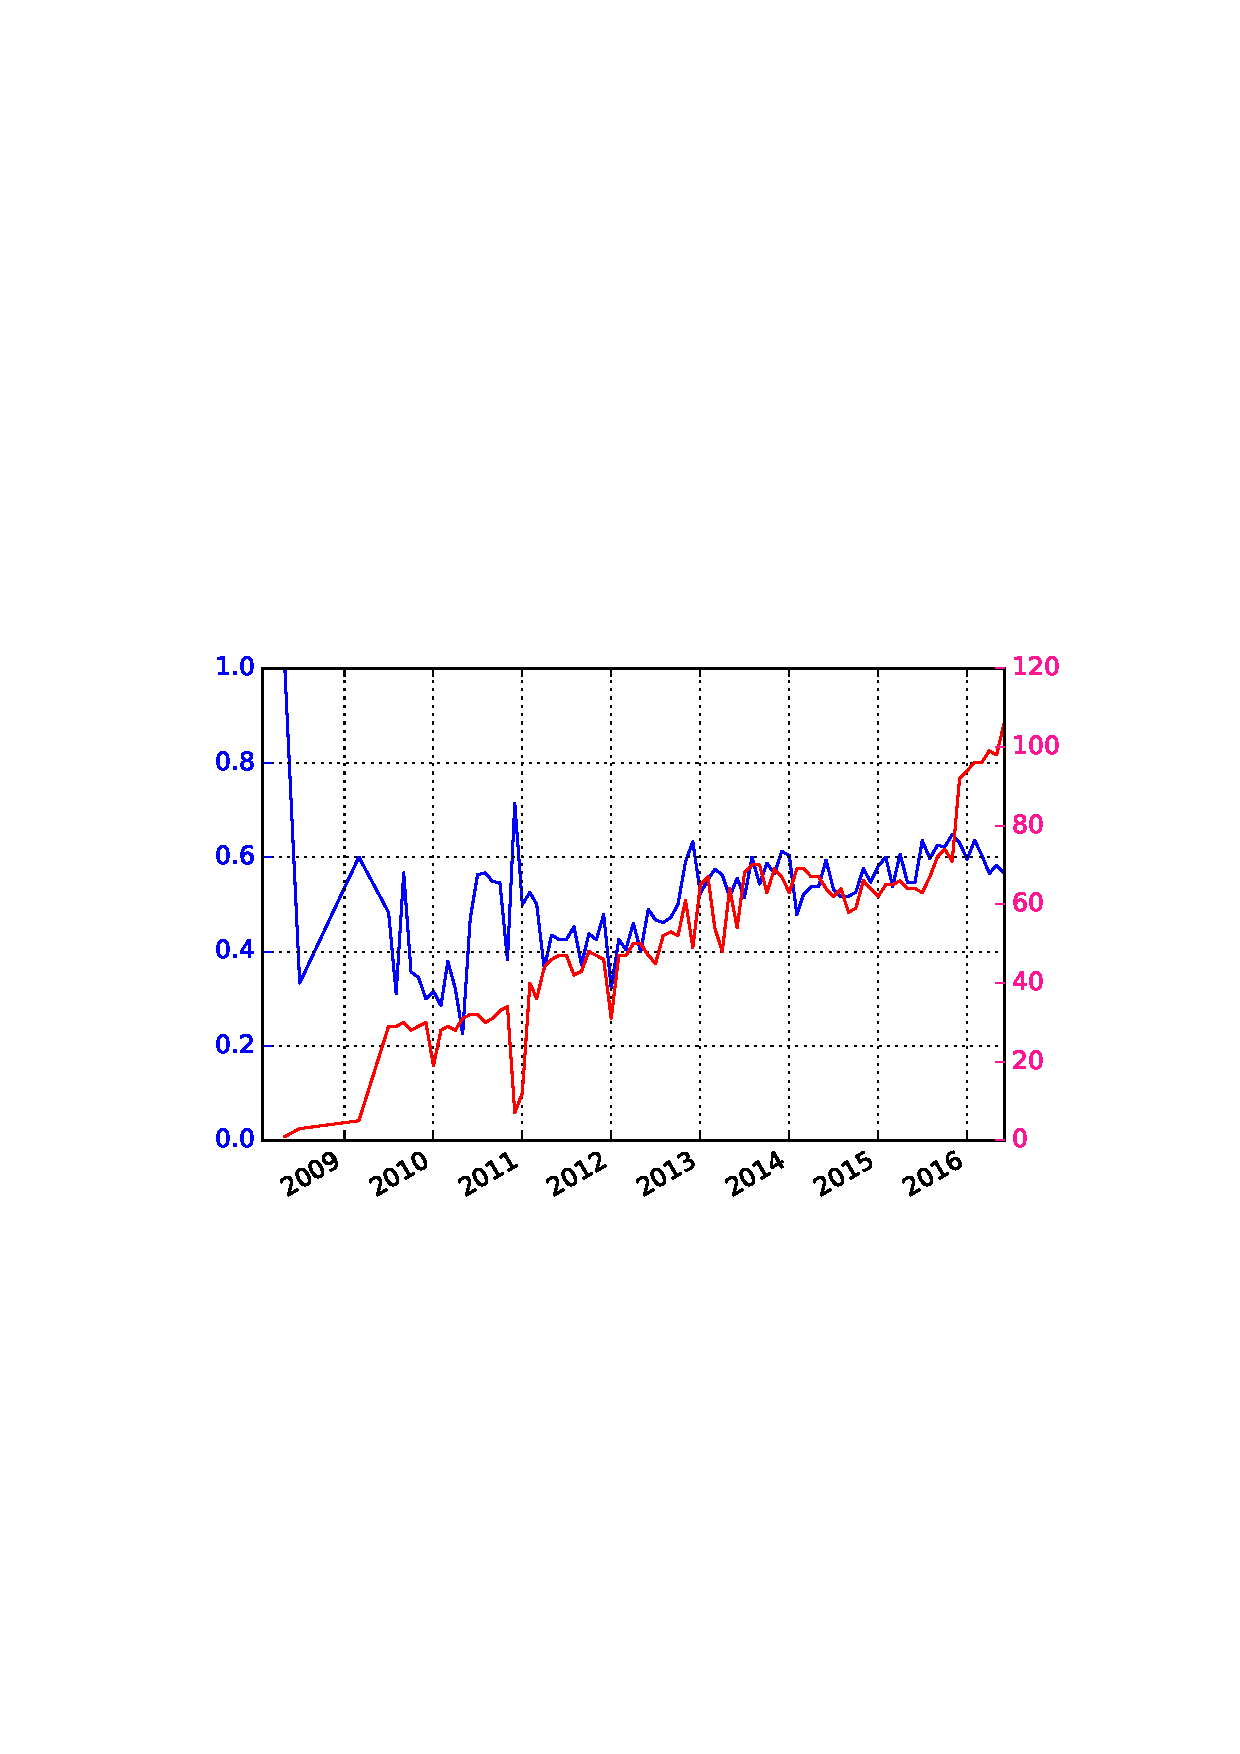
\includegraphics[width=\linewidth]{img/convergence_over_time_l.png}
			\caption{L-Root}
			\label{fig:convergence-l}
		\end{subfigure}											
		\begin{subfigure}{.32\textwidth}
			\centering
			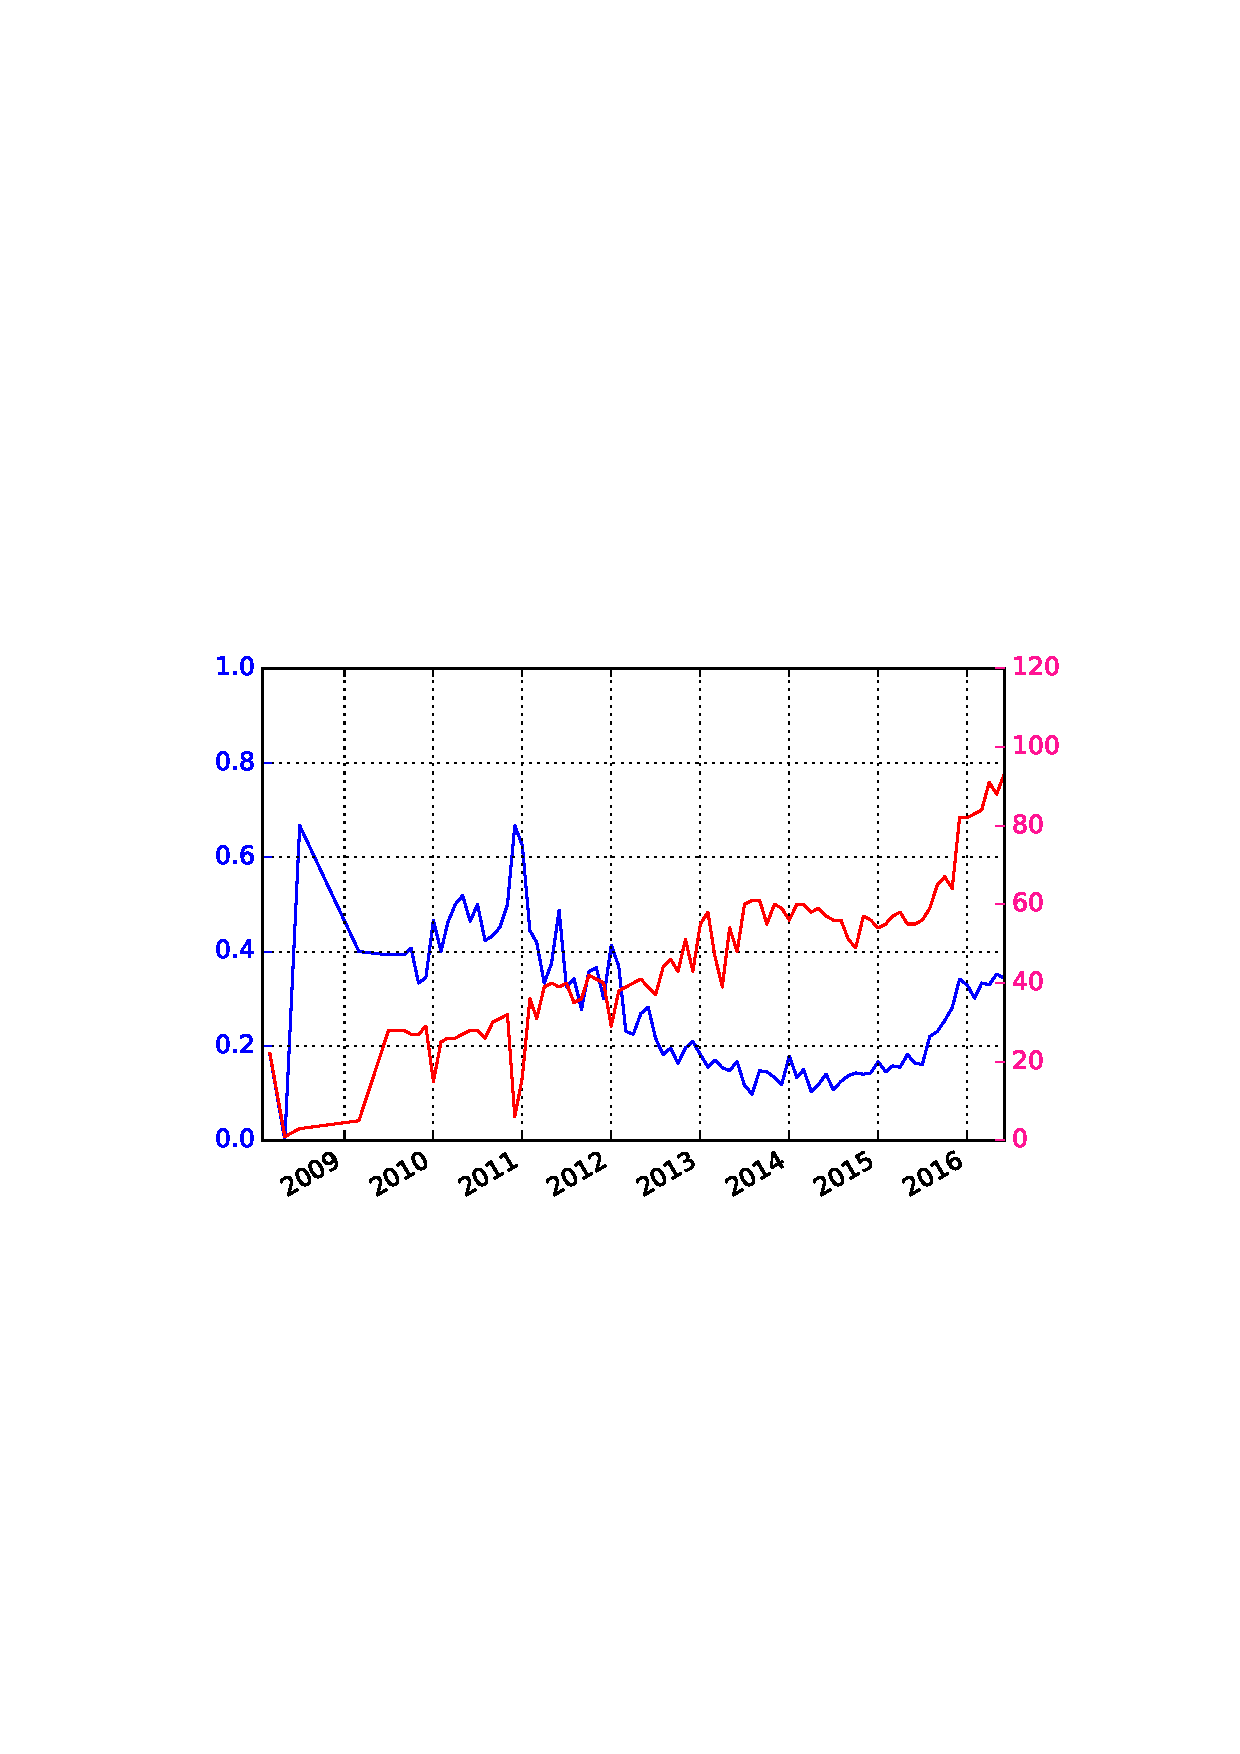
\includegraphics[width=\linewidth]{img/convergence_over_time_m.png}
			\caption{M-Root}
			\label{fig:app:convergence-m}
		\end{subfigure}
		\caption{Convergence level}
		\label{fig:app:convergence}	
	\end{figure}
	

	
	\chapter{VPs Composition}
	\label{app:peer-composition}
	A mutual VP can have either diverging or converging IPv4/IPv6 paths. For diverging paths, it can be: \textit{(i)} have shorter IPv4 path, \textit{(ii)} have shorter IPv6 path, or \textit{(iii)} have equal path length. The following graphs represent the VPs composition in terms of the aforementioned categorization for each Root Server. To provide better readability, the height of each stacked bar is normalized and the total number of VPs per time is displayed at the top of the graph.
	
	\begin{figure}[!htb]
		\centering
		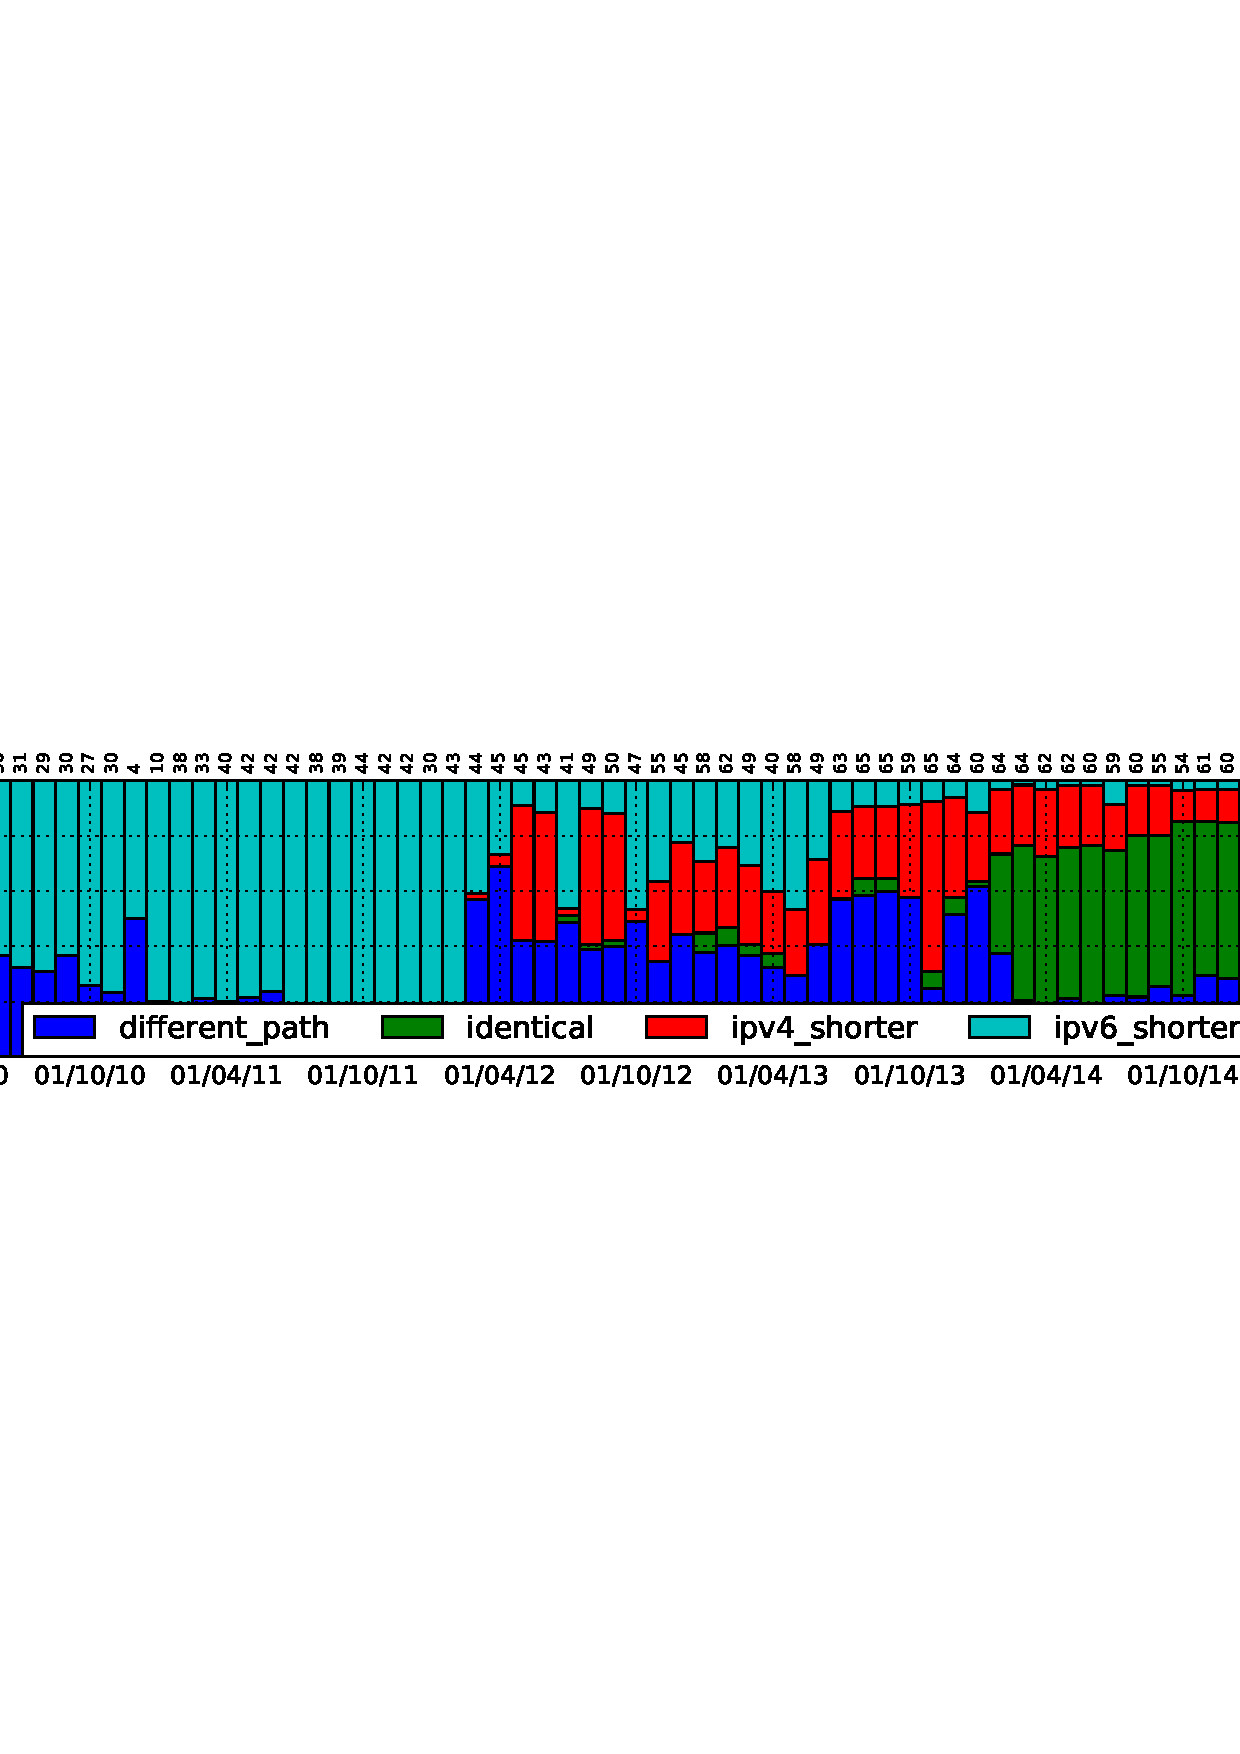
\includegraphics[width=6.0in]{img/peer_composition_a.png}
		\caption{A-Root peers composition}
		\label{fig:peer-comp-a}
	\end{figure}
	\begin{figure}[!htb]
		\centering
		\includegraphics[width=6.0in]{img/peer_composition_c.png}
		\caption{C-Root VPs composition}
		\label{fig:peer-comp-c}
	\end{figure}
	\begin{figure}[!htb]
		\centering
		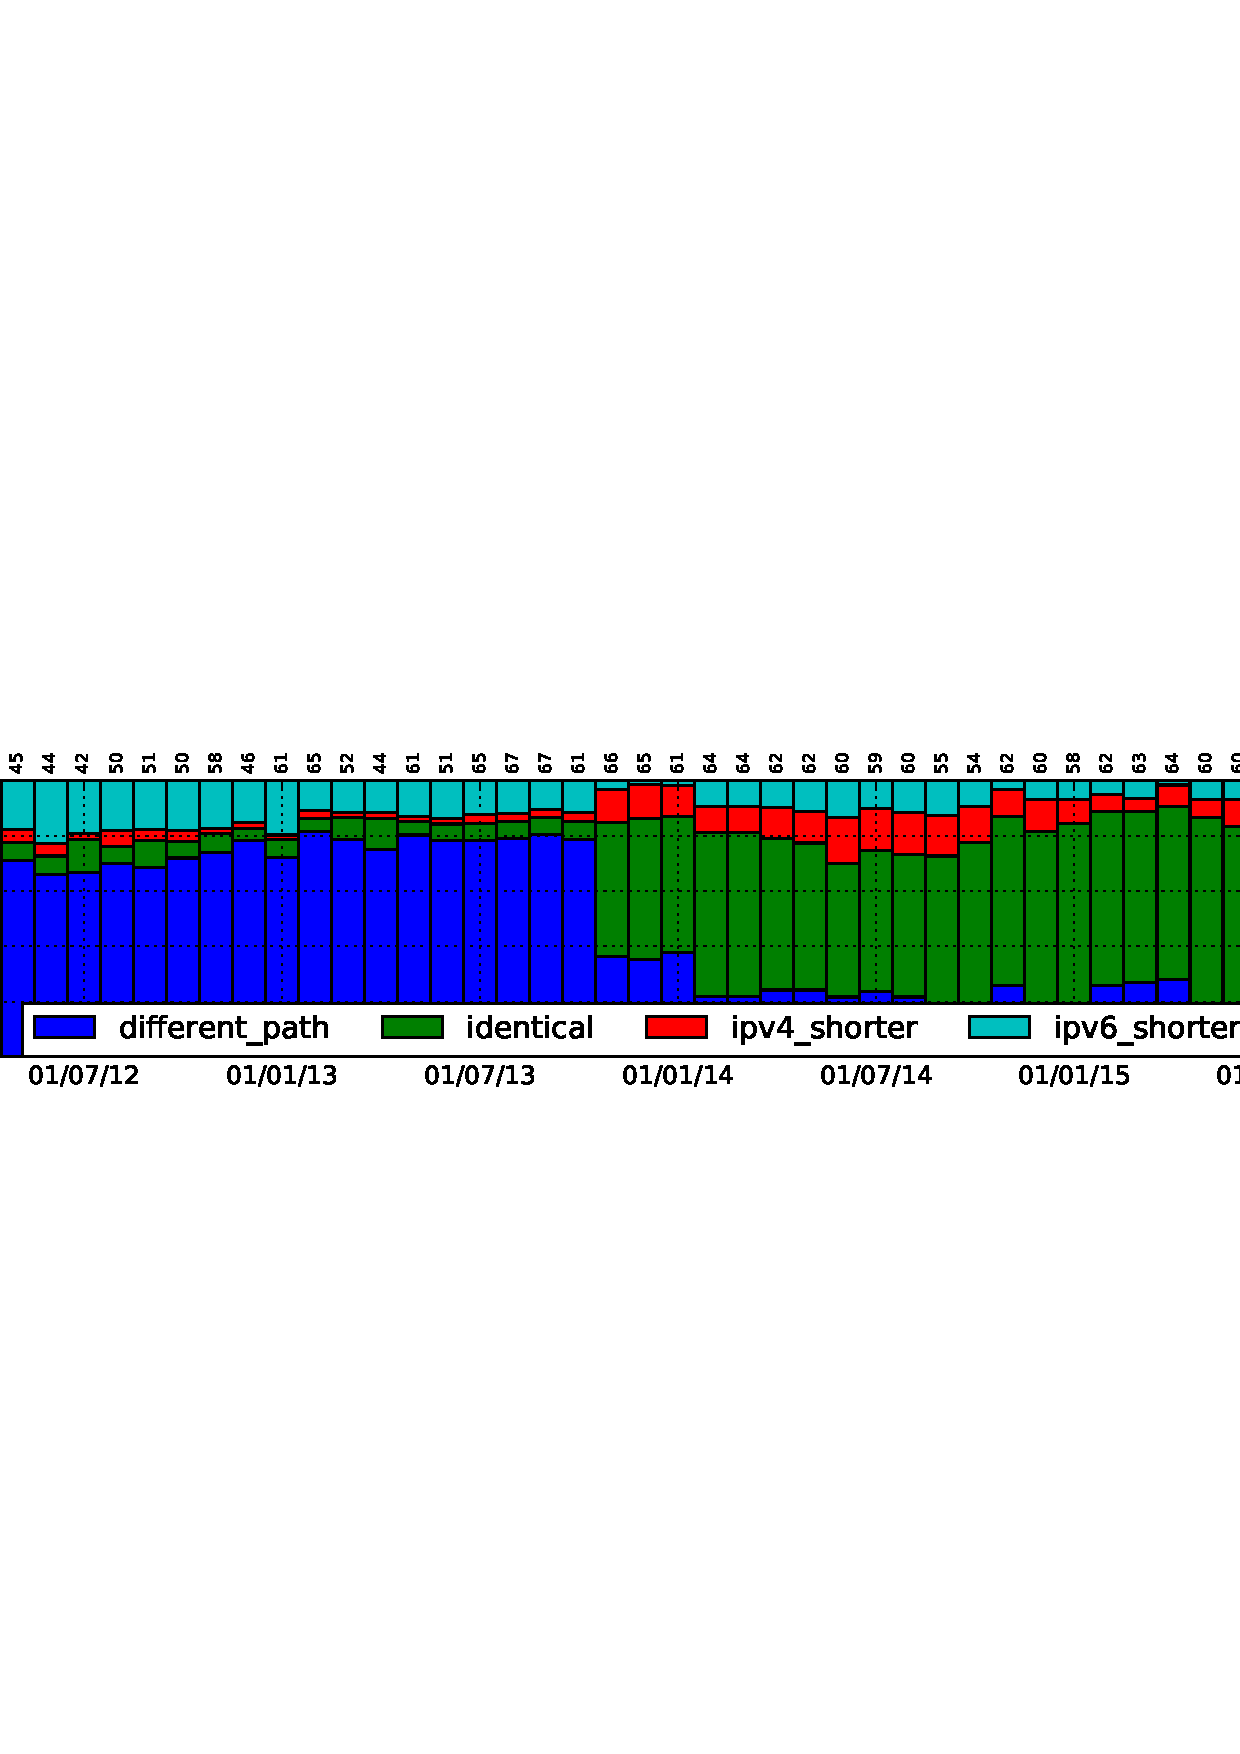
\includegraphics[width=6.0in]{img/peer_composition_d.png}
		\caption{D-Root VPs composition}
		\label{fig:peer-comp-d}
	\end{figure}
	\begin{figure}[!htb]
		\centering
		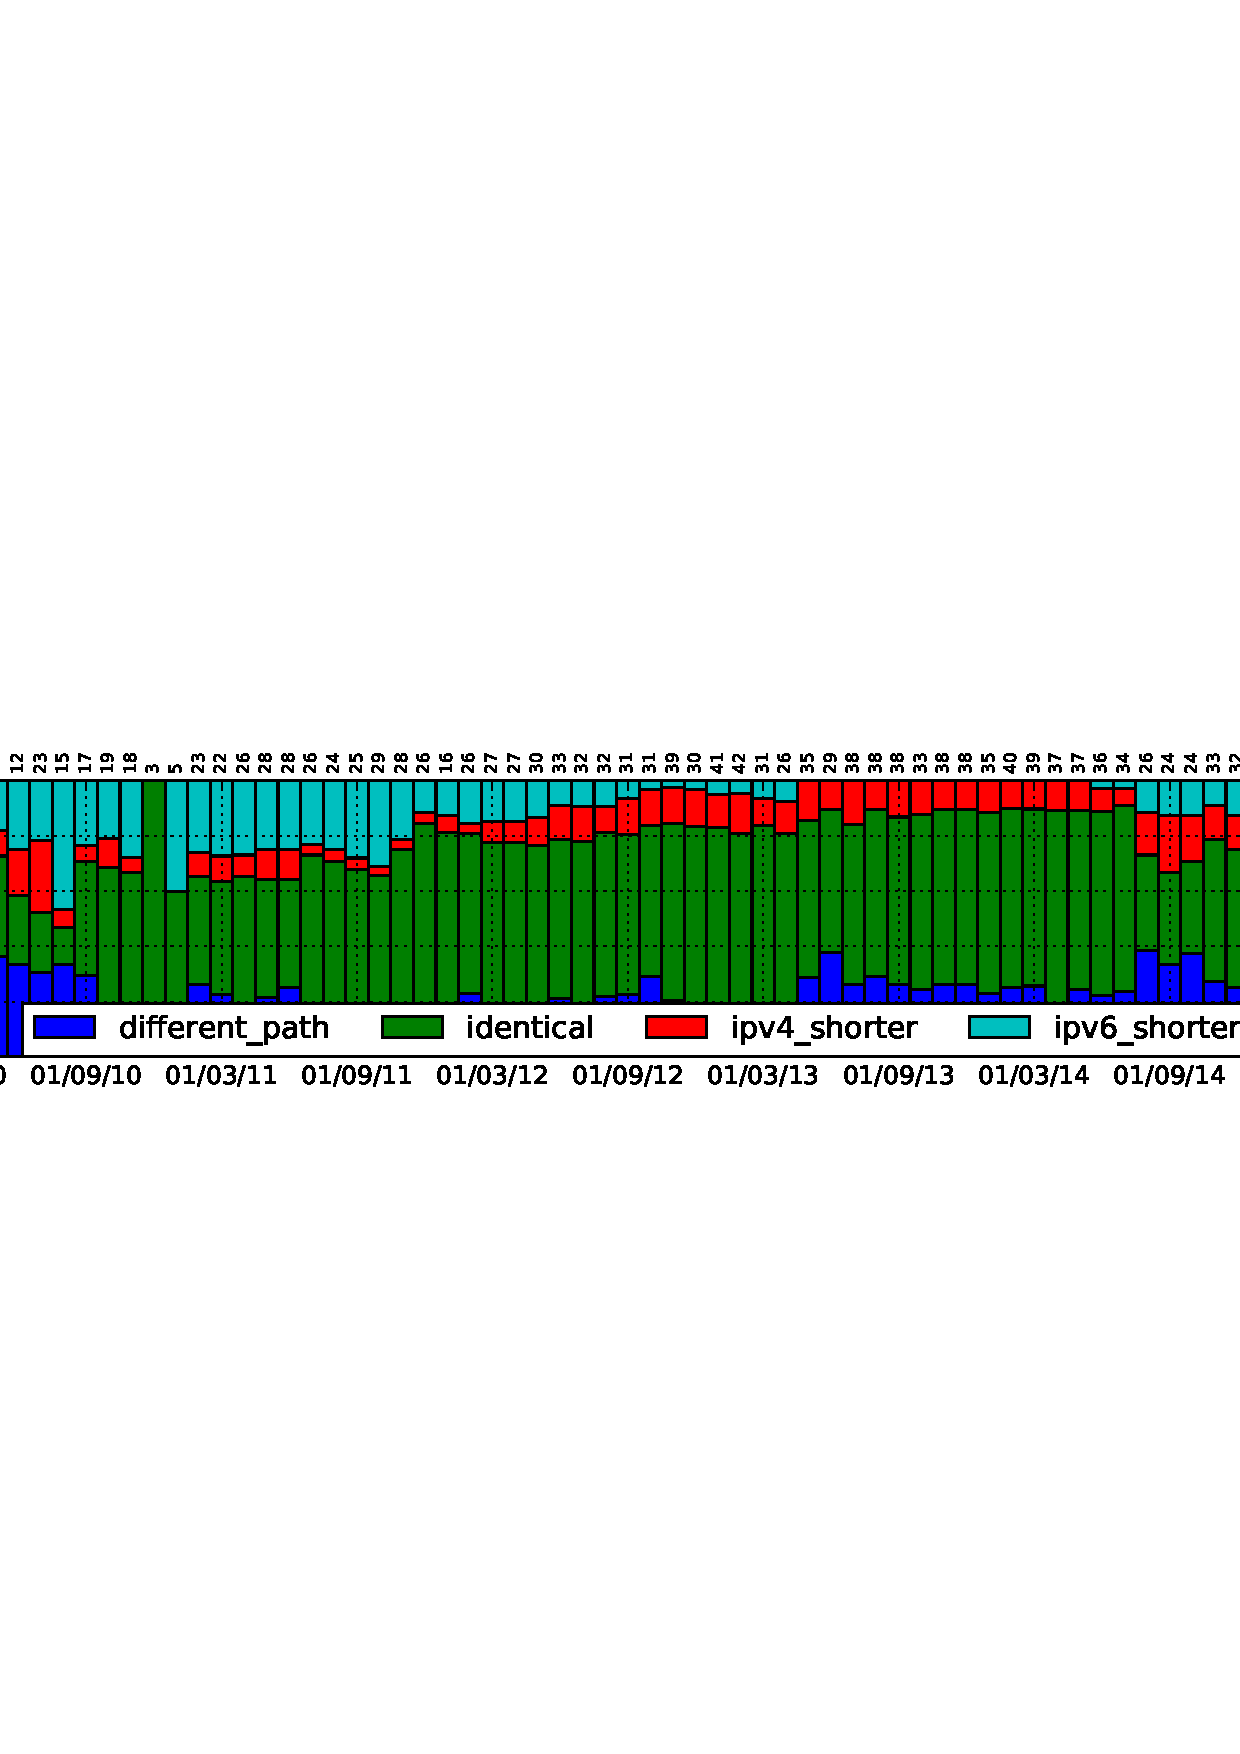
\includegraphics[width=6.0in]{img/peer_composition_f.png}
		\caption{F-Root VPs composition}
		\label{fig:peer-comp-f}
	\end{figure}
	\begin{figure}[!htb]
		\centering
		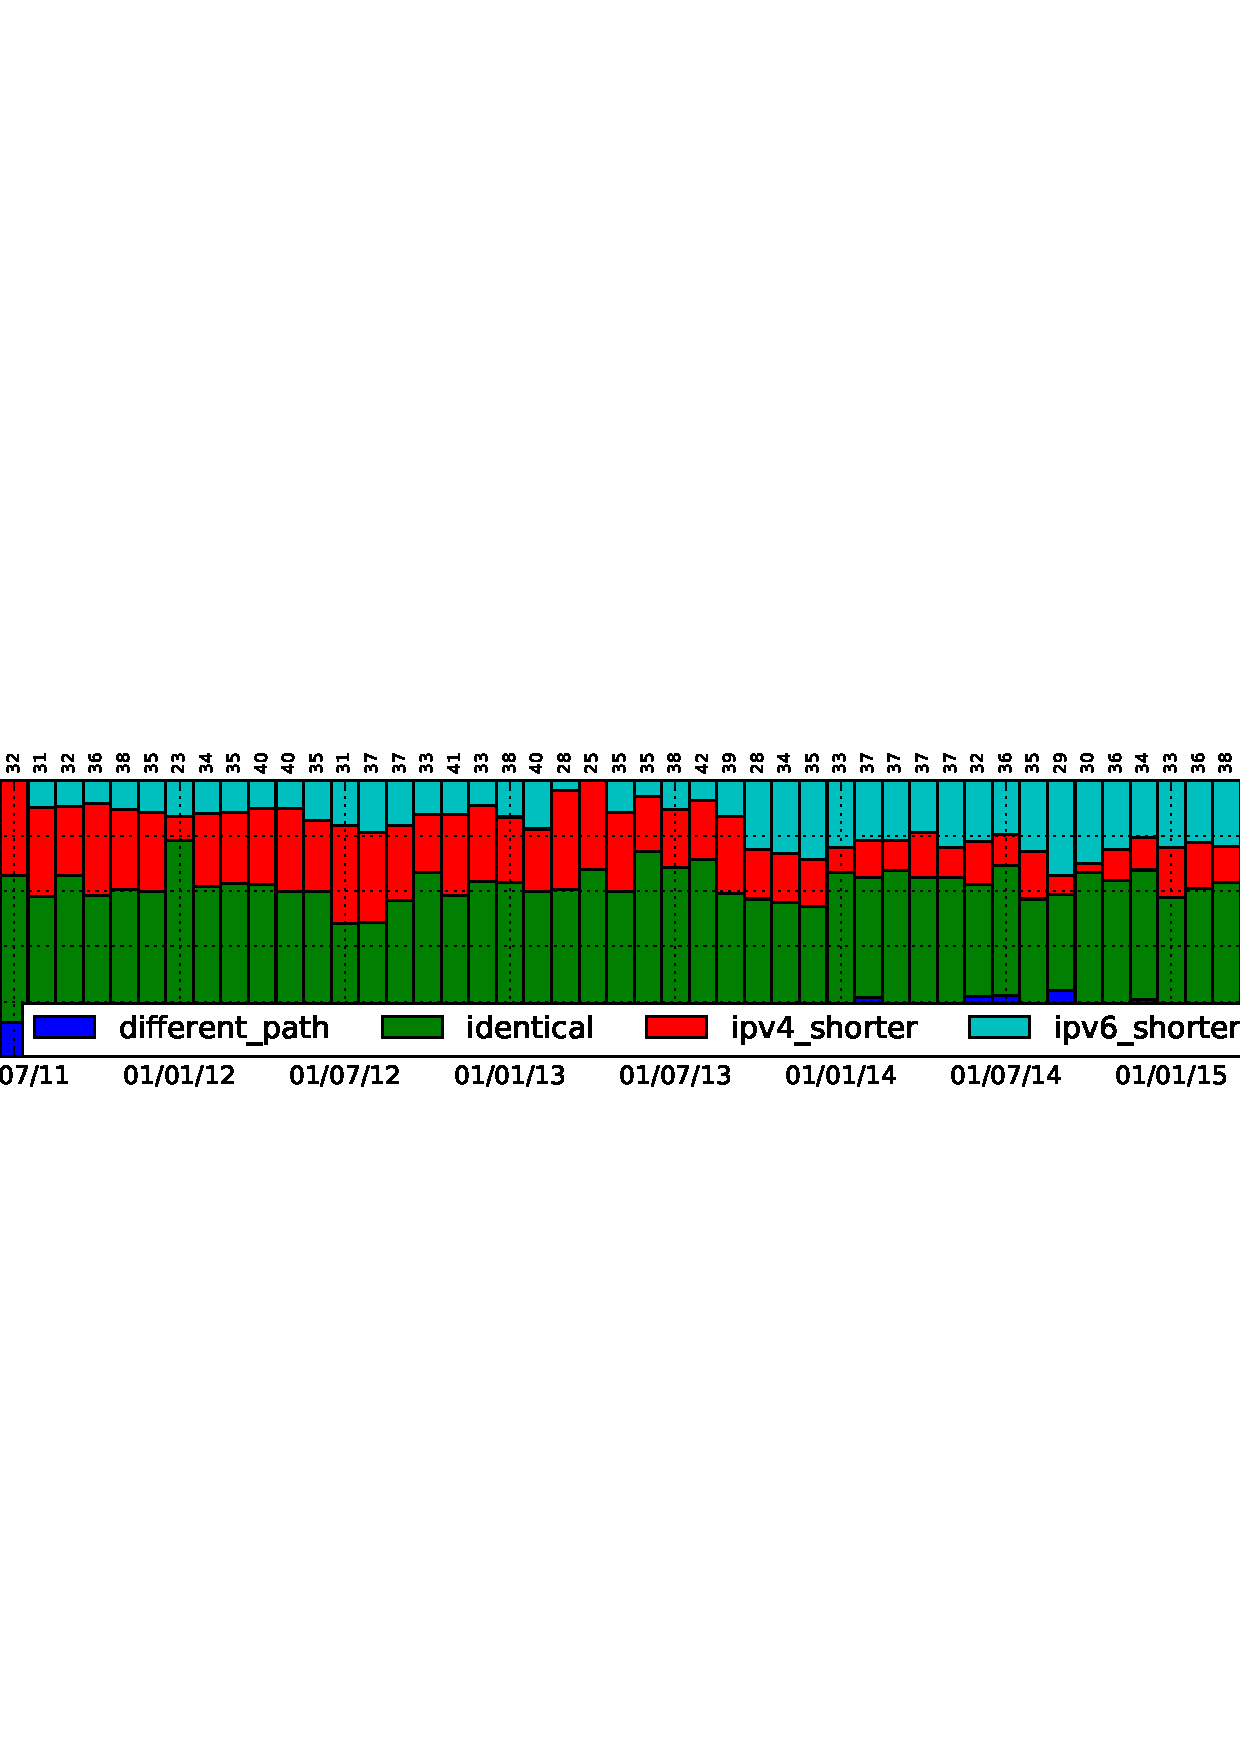
\includegraphics[width=6.0in]{img/peer_composition_i.png}
		\caption{I-Root VPs composition}
		\label{fig:peer-comp-i}
	\end{figure}
	\begin{figure}[!htb]
		\centering
		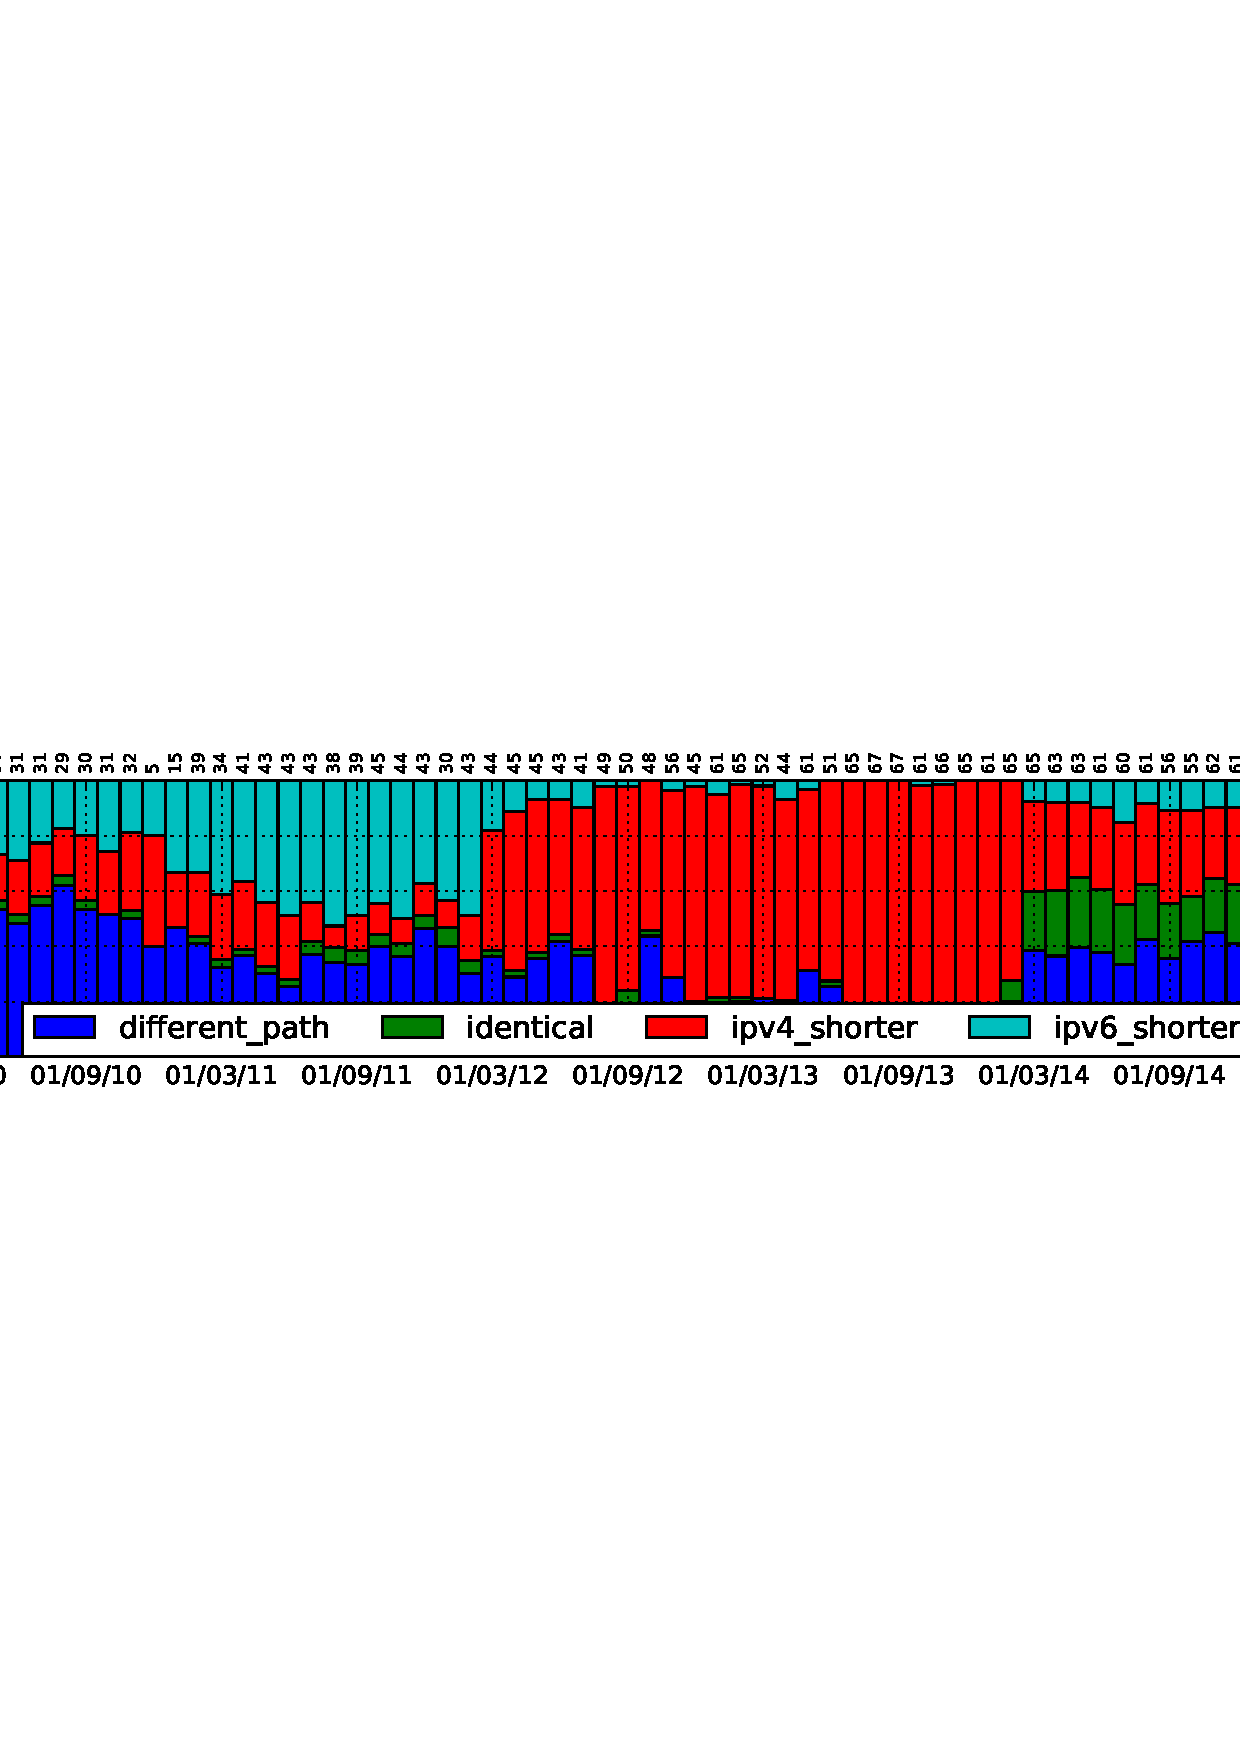
\includegraphics[width=6.0in]{img/peer_composition_j.png}
		\caption{J-Root VPs composition}
		\label{fig:peer-comp-j}
	\end{figure}
	\begin{figure}[!htb]
		\centering
		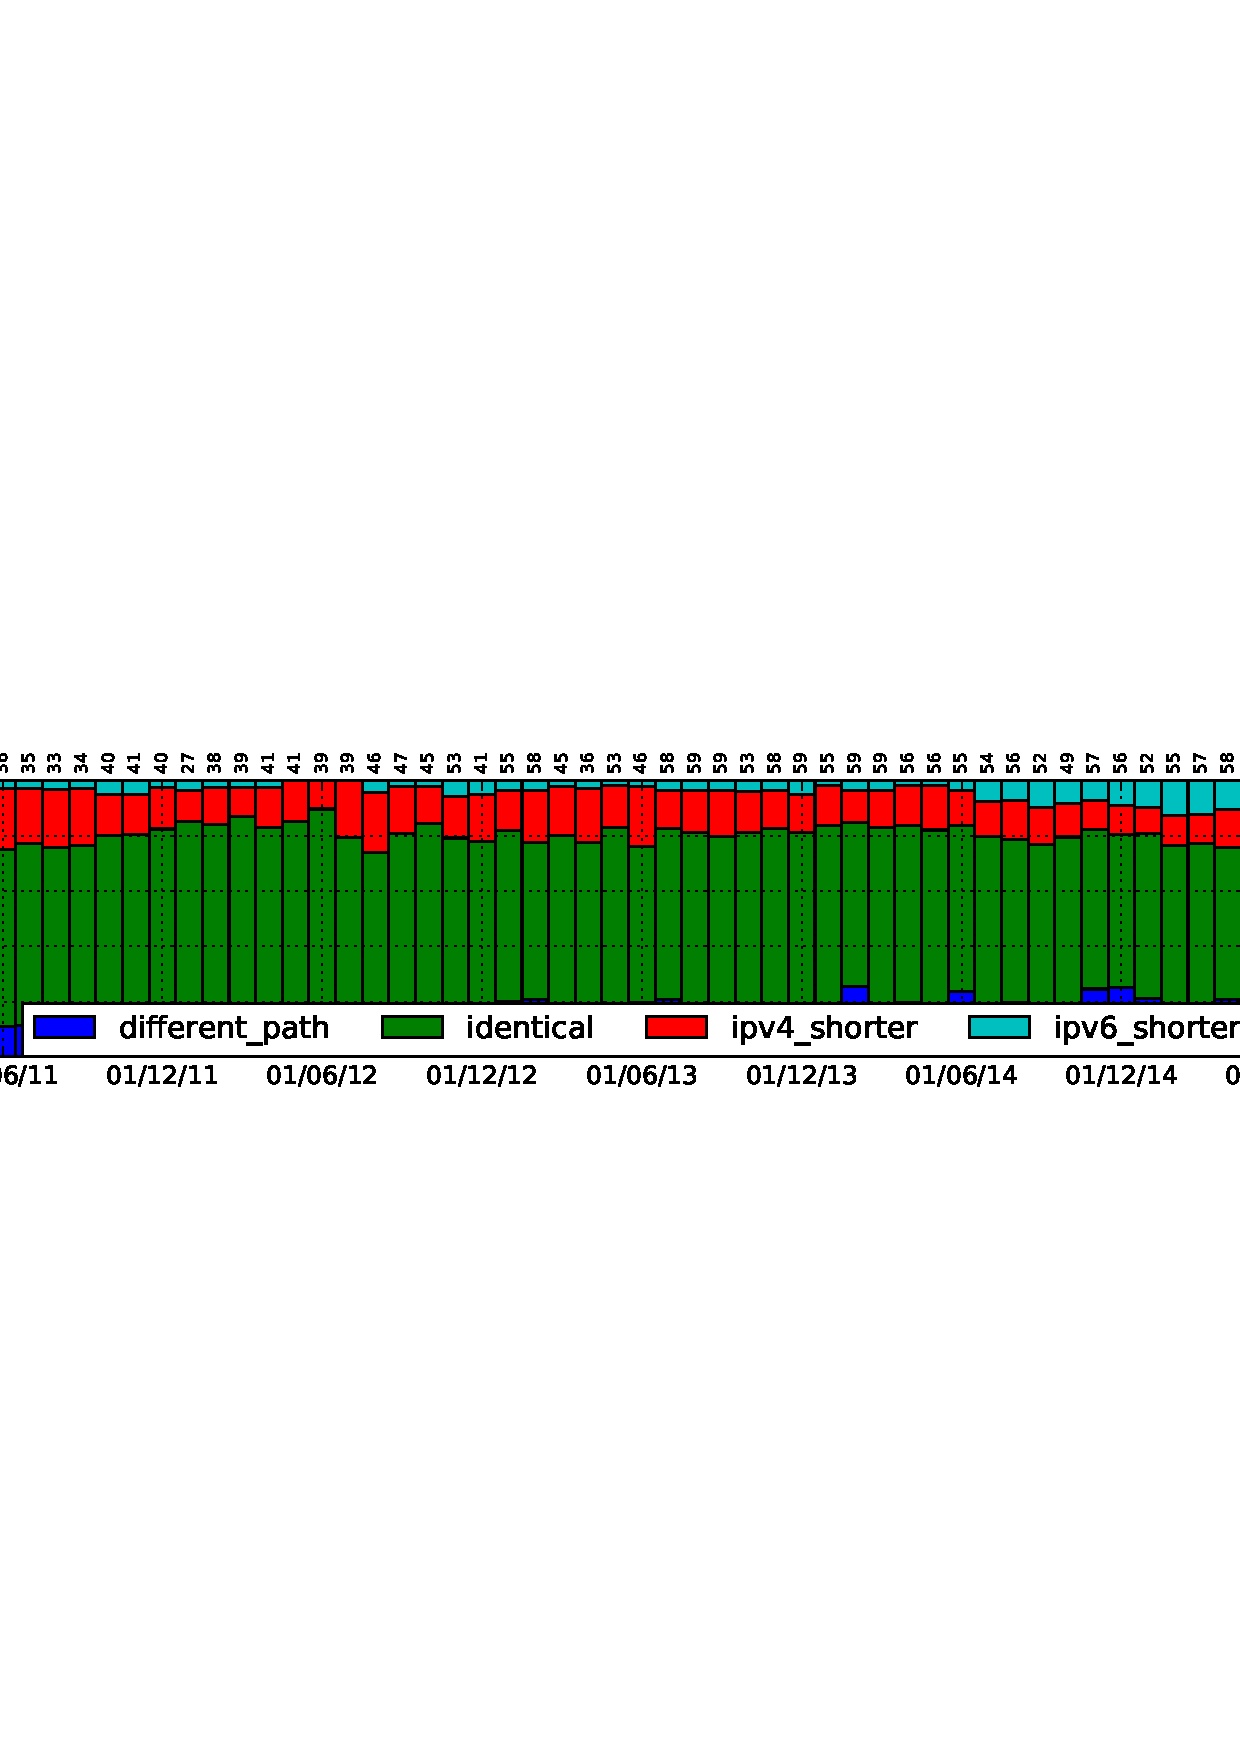
\includegraphics[width=6.0in]{img/peer_composition_k.png}
		\caption{K-Root VPs composition}
		\label{fig:peer-comp-k}
	\end{figure}
	\begin{figure}[!htb]
		\centering
		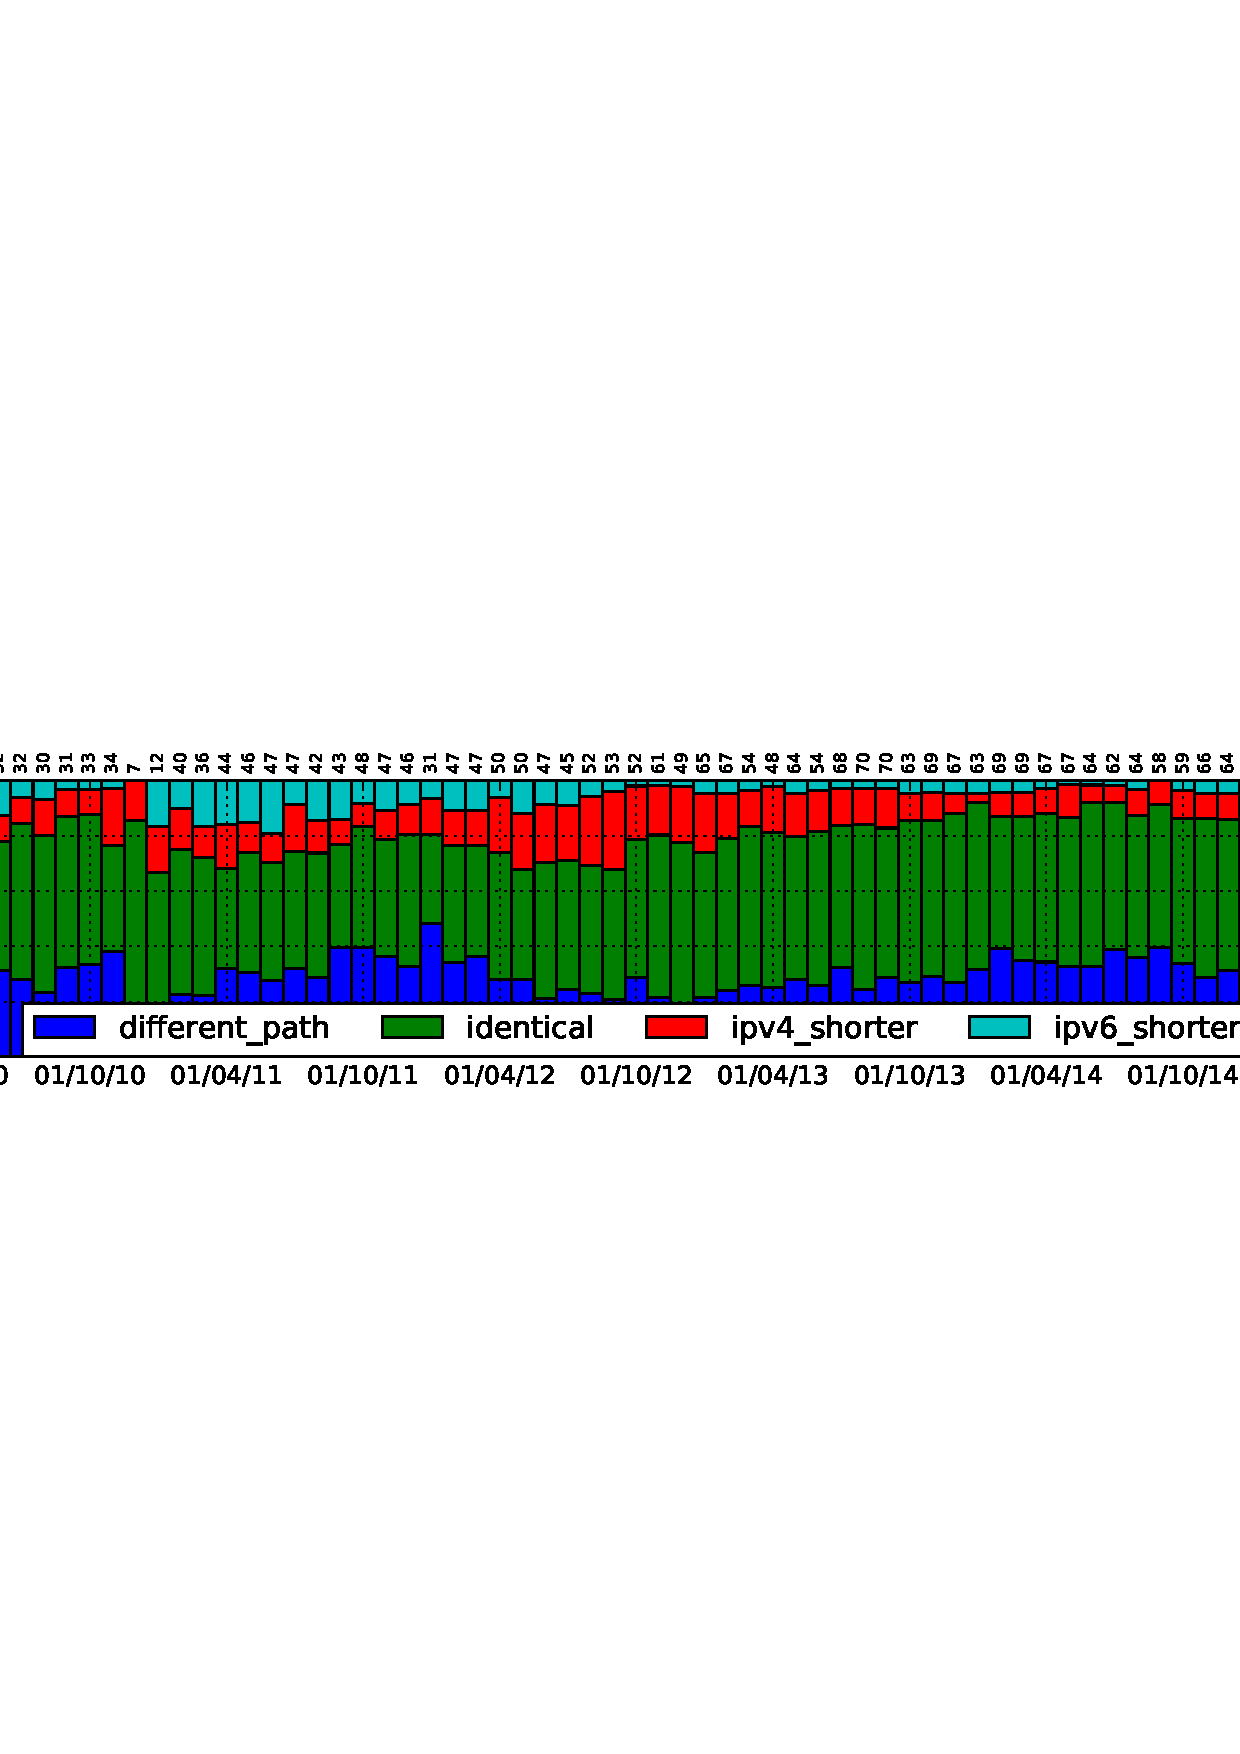
\includegraphics[width=6.0in]{img/peer_composition_l.png}
		\caption{L-Root VPs composition}
		\label{fig:peer-comp-l}
	\end{figure}
	\begin{figure}[!htb]
		\centering
		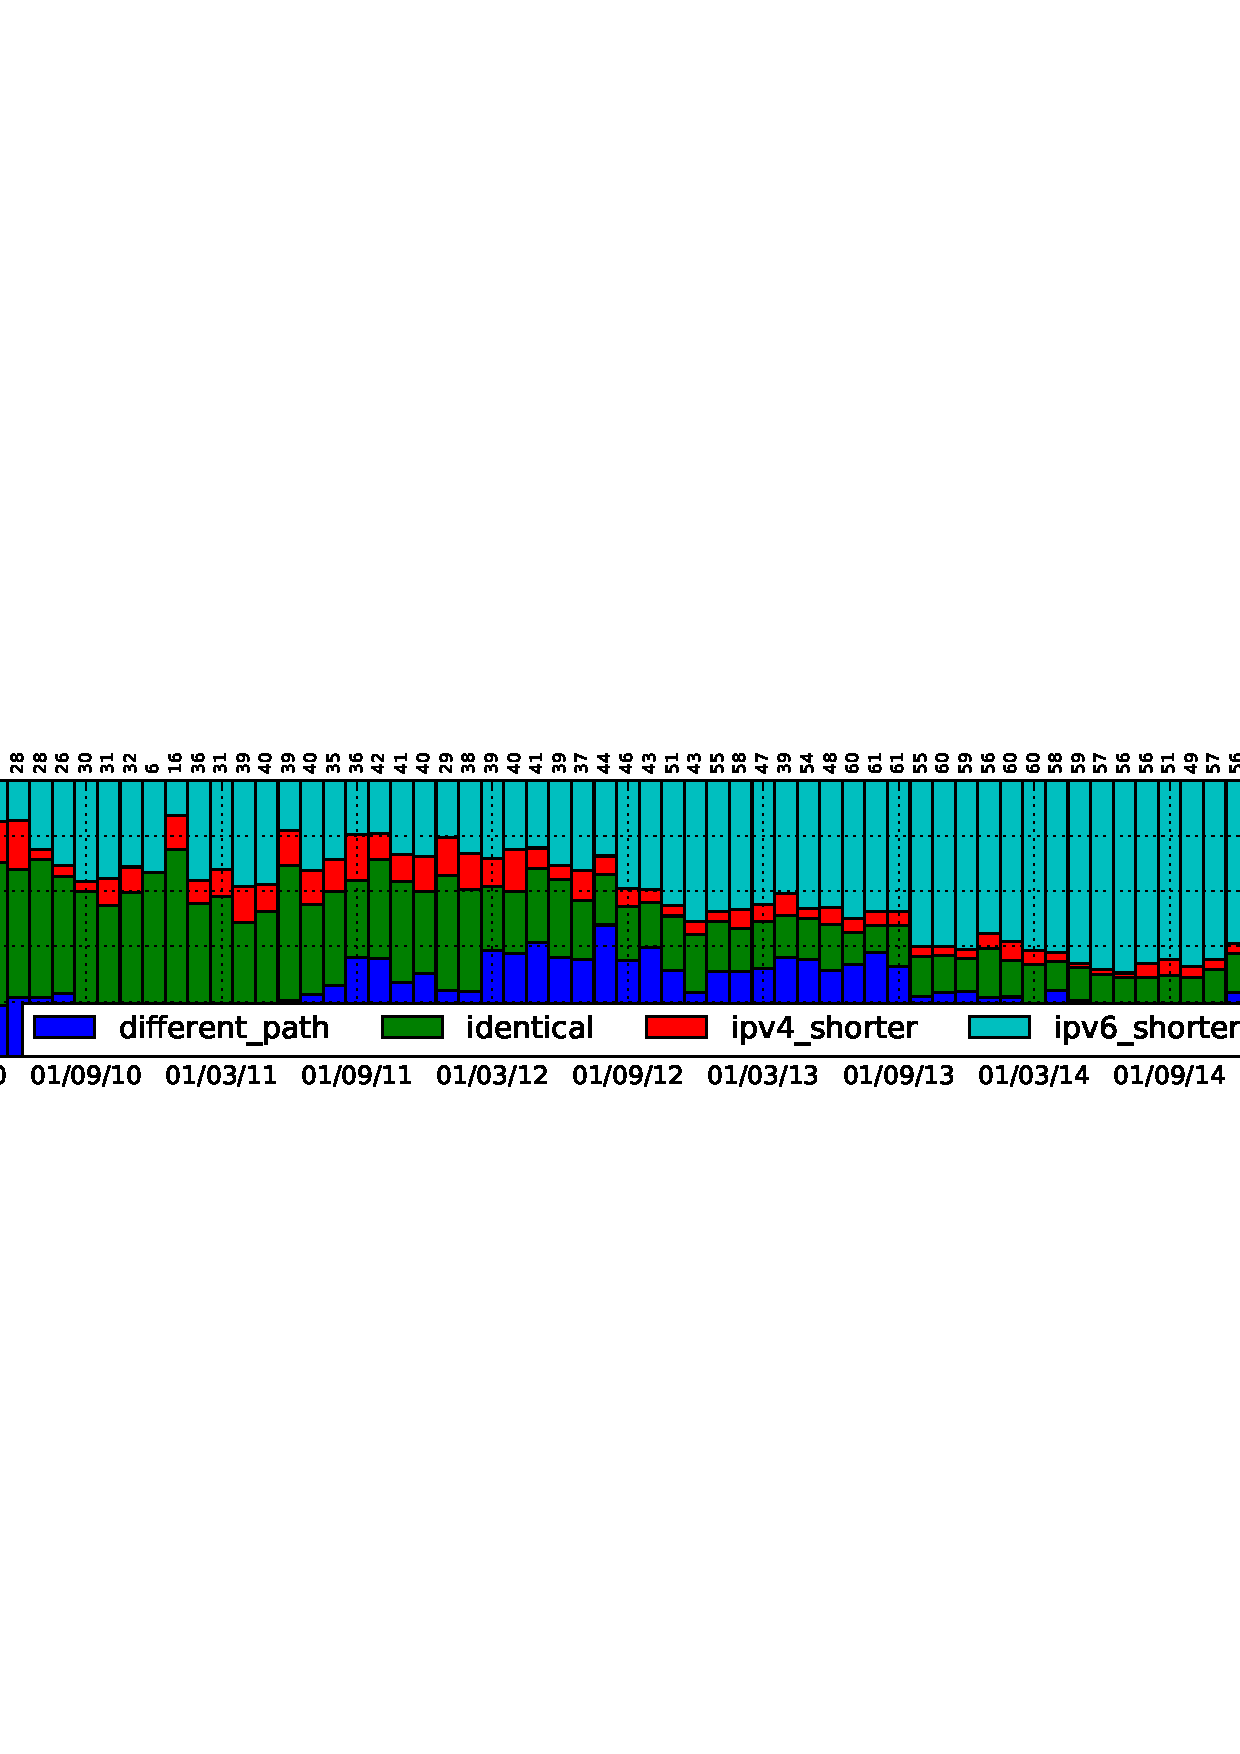
\includegraphics[width=6.0in]{img/peer_composition_m.png}
		\caption{M-Root VPs composition}
		\label{fig:peer-comp-m}
	\end{figure}
	
	\chapter{AS Path Length Distribution}
	\label{app:path-avg}
	
	The box plot is generated using Matplotlib with default configuration. The closed box comprising of three horizontally parallel lines represents the 1\textsuperscript{st} quartile, the median, and the 3\textsuperscript{rd} quartile (bottom to top). Interquartile range (IQR) is defined as the range between 1\textsuperscript{st} quartile and 3\textsuperscript{rd} quartile. The top whisker represents the maximum value below 75\% + 1.5 IQR, while the bottom one represents the minimum value above 25\% - 1.5 IQR. Any value falls outside those boundaries are regarded as outlier (plotted as '+'). The green line represents the median of all path length values over the time.
	
	Appendix \ref{app:path-avg:all-peers} represents AS path length distribution for all mutual VPs, regardless diverging or converging. Appendix \ref{app:path-avg:diff-paths} represents the distribution only for diverging VPs.
	\section{All VPs}
	\label{app:path-avg:all-peers}
		\begin{figure}[!htb]
			\centering
			\includegraphics[width=6.0in]{img/path_avg_all_a.png}
			\caption{Path average length of all peers of A-Root}
			\label{fig:path-avg-all-a}
		\end{figure}
		\begin{figure}[!htb]
			\centering
			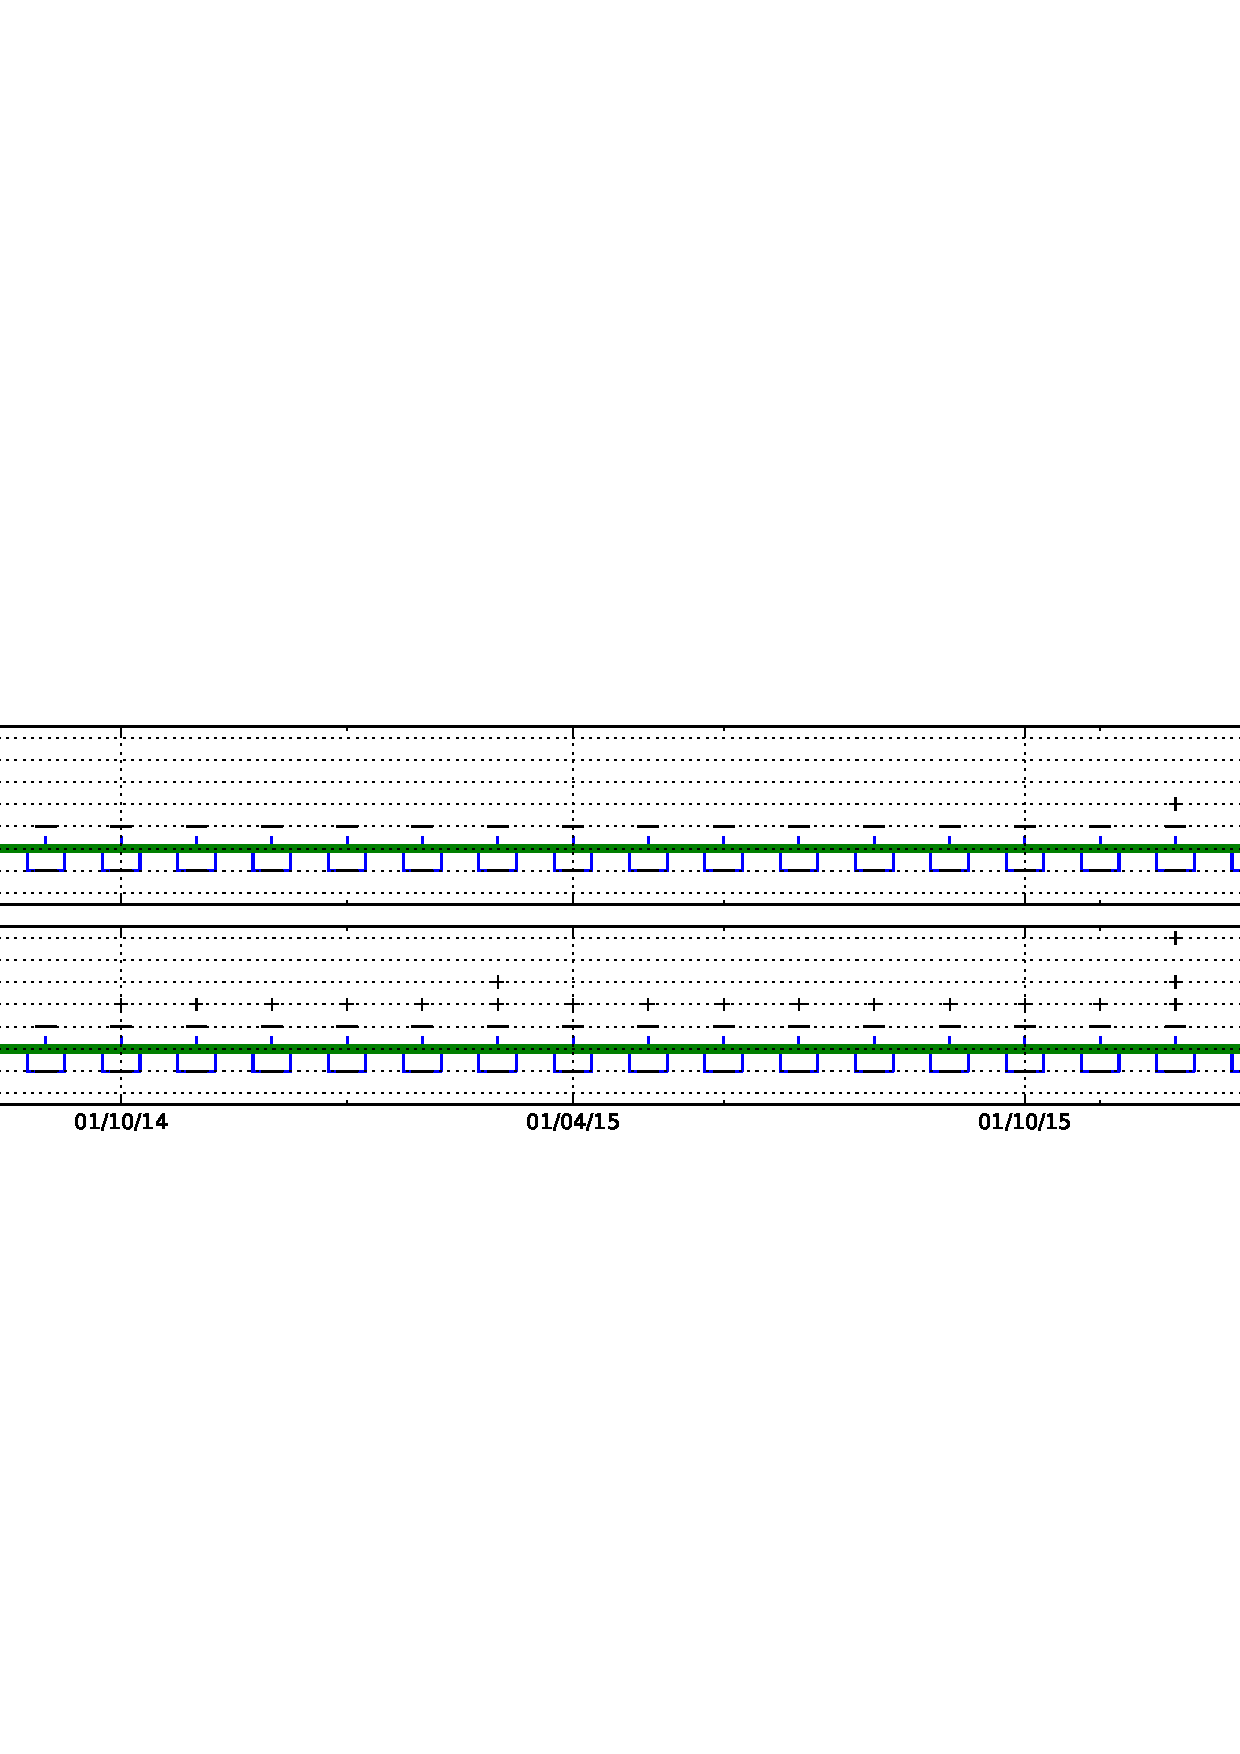
\includegraphics[width=6.0in]{img/path_avg_all_c.png}
			\caption{Path length distribution of all C-Root's VPs}
			\label{fig:path-avg-all-c}
		\end{figure}
		\begin{figure}[!htb]
			\centering
			\includegraphics[width=6.0in]{img/path_avg_all_d.png}
			\caption{Path length distribution of all D-Root's VPs}
			\label{fig:path-avg-all-d}
		\end{figure}
		\begin{figure}[!htb]
			\centering
			\includegraphics[width=6.0in]{img/path_avg_all_f.png}
			\caption{Path length distribution of all F-Root's VPs}
			\label{fig:path-avg-all-f}
		\end{figure}
		
		\begin{figure}[!htb]
			\centering
			\includegraphics[width=6.0in]{img/path_avg_all_i.png}
			\caption{Path length distribution of all I-Root's VPs}
			\label{fig:path-avg-all-i}
		\end{figure}
		
		\begin{figure}[!htb]
			\centering
			\includegraphics[width=6.0in]{img/path_avg_all_j.png}
			\caption{Path length distribution of all J-Root's VPs}
			\label{fig:path-avg-all-j}
		\end{figure}
		\begin{figure}[!htb]
			\centering
			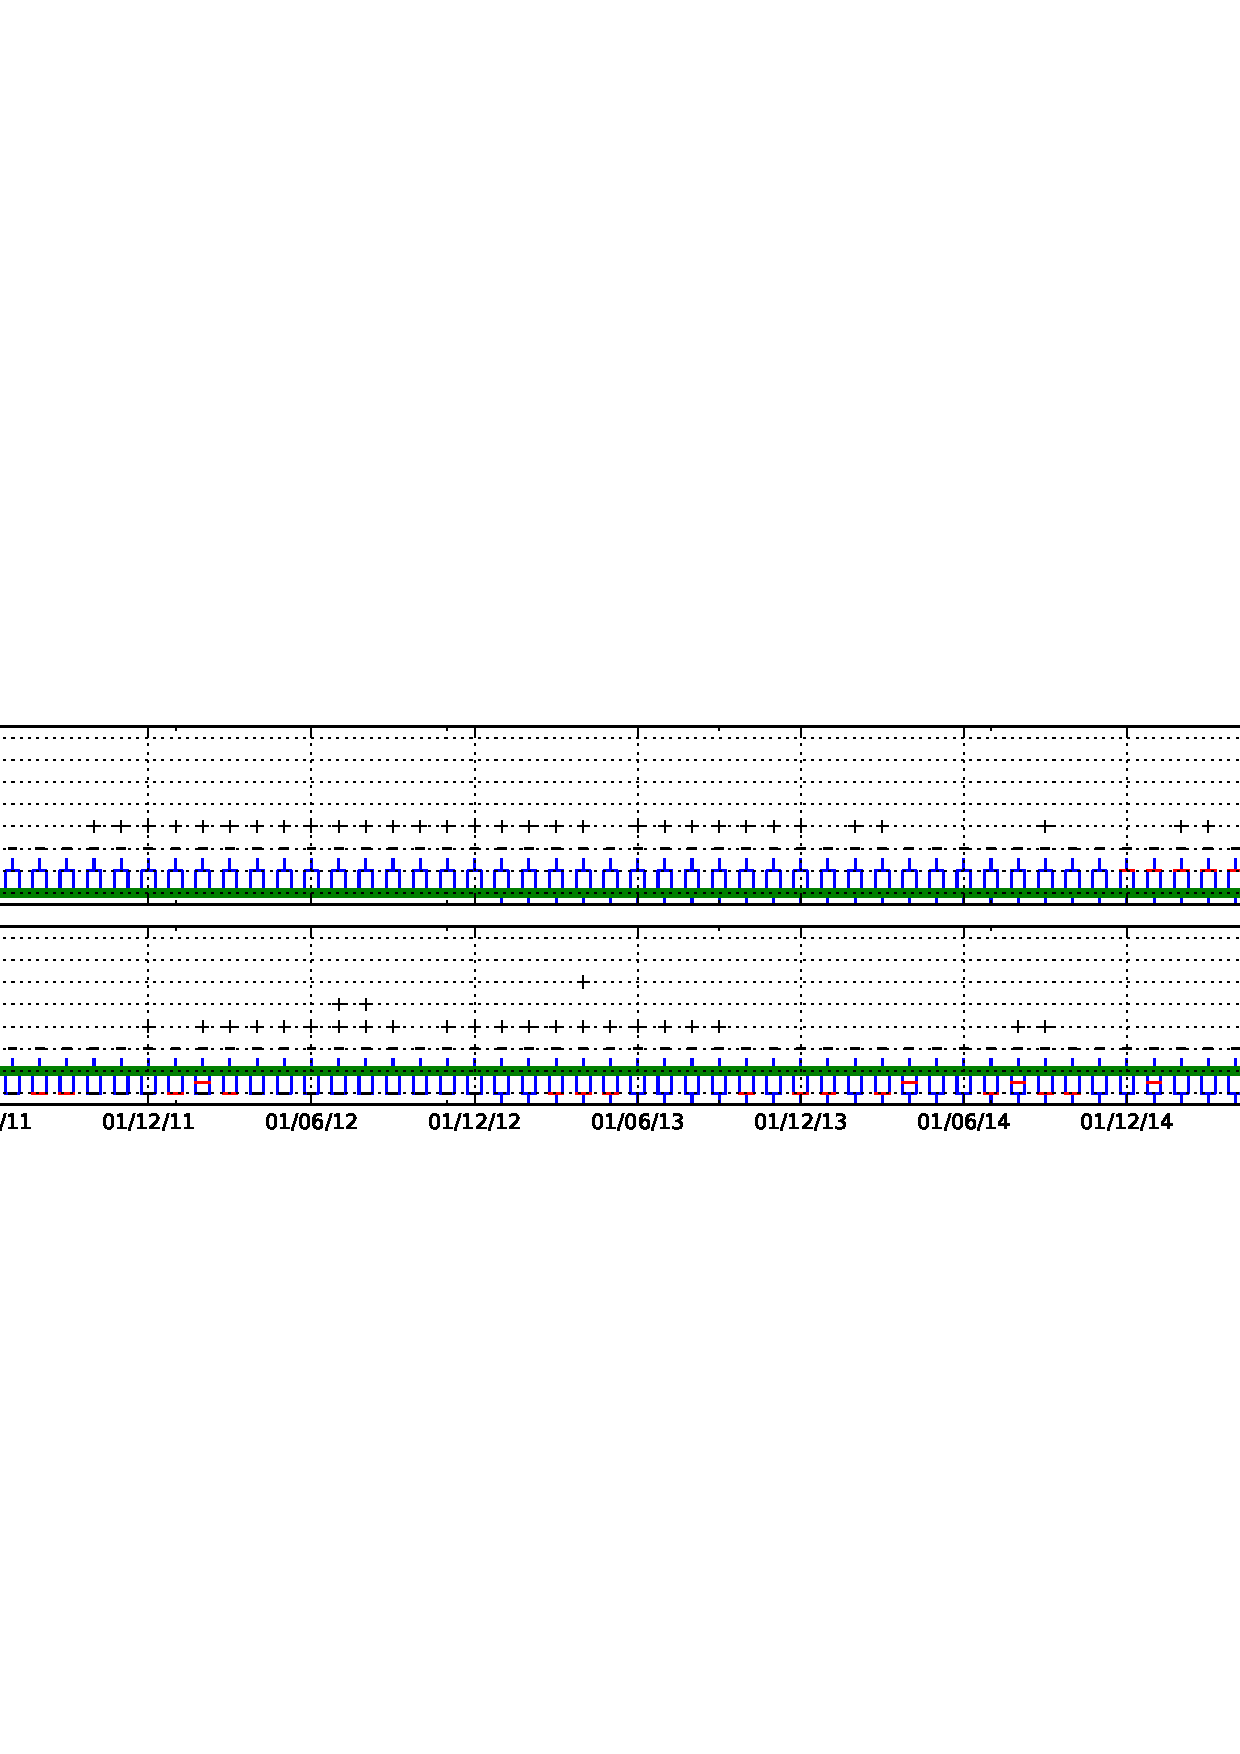
\includegraphics[width=6.0in]{img/path_avg_all_k.png}
			\caption{Path length distribution of all K-Root's VPs}
			\label{fig:path-avg-all-k}
		\end{figure}
		\begin{figure}[!htb]
			\centering
			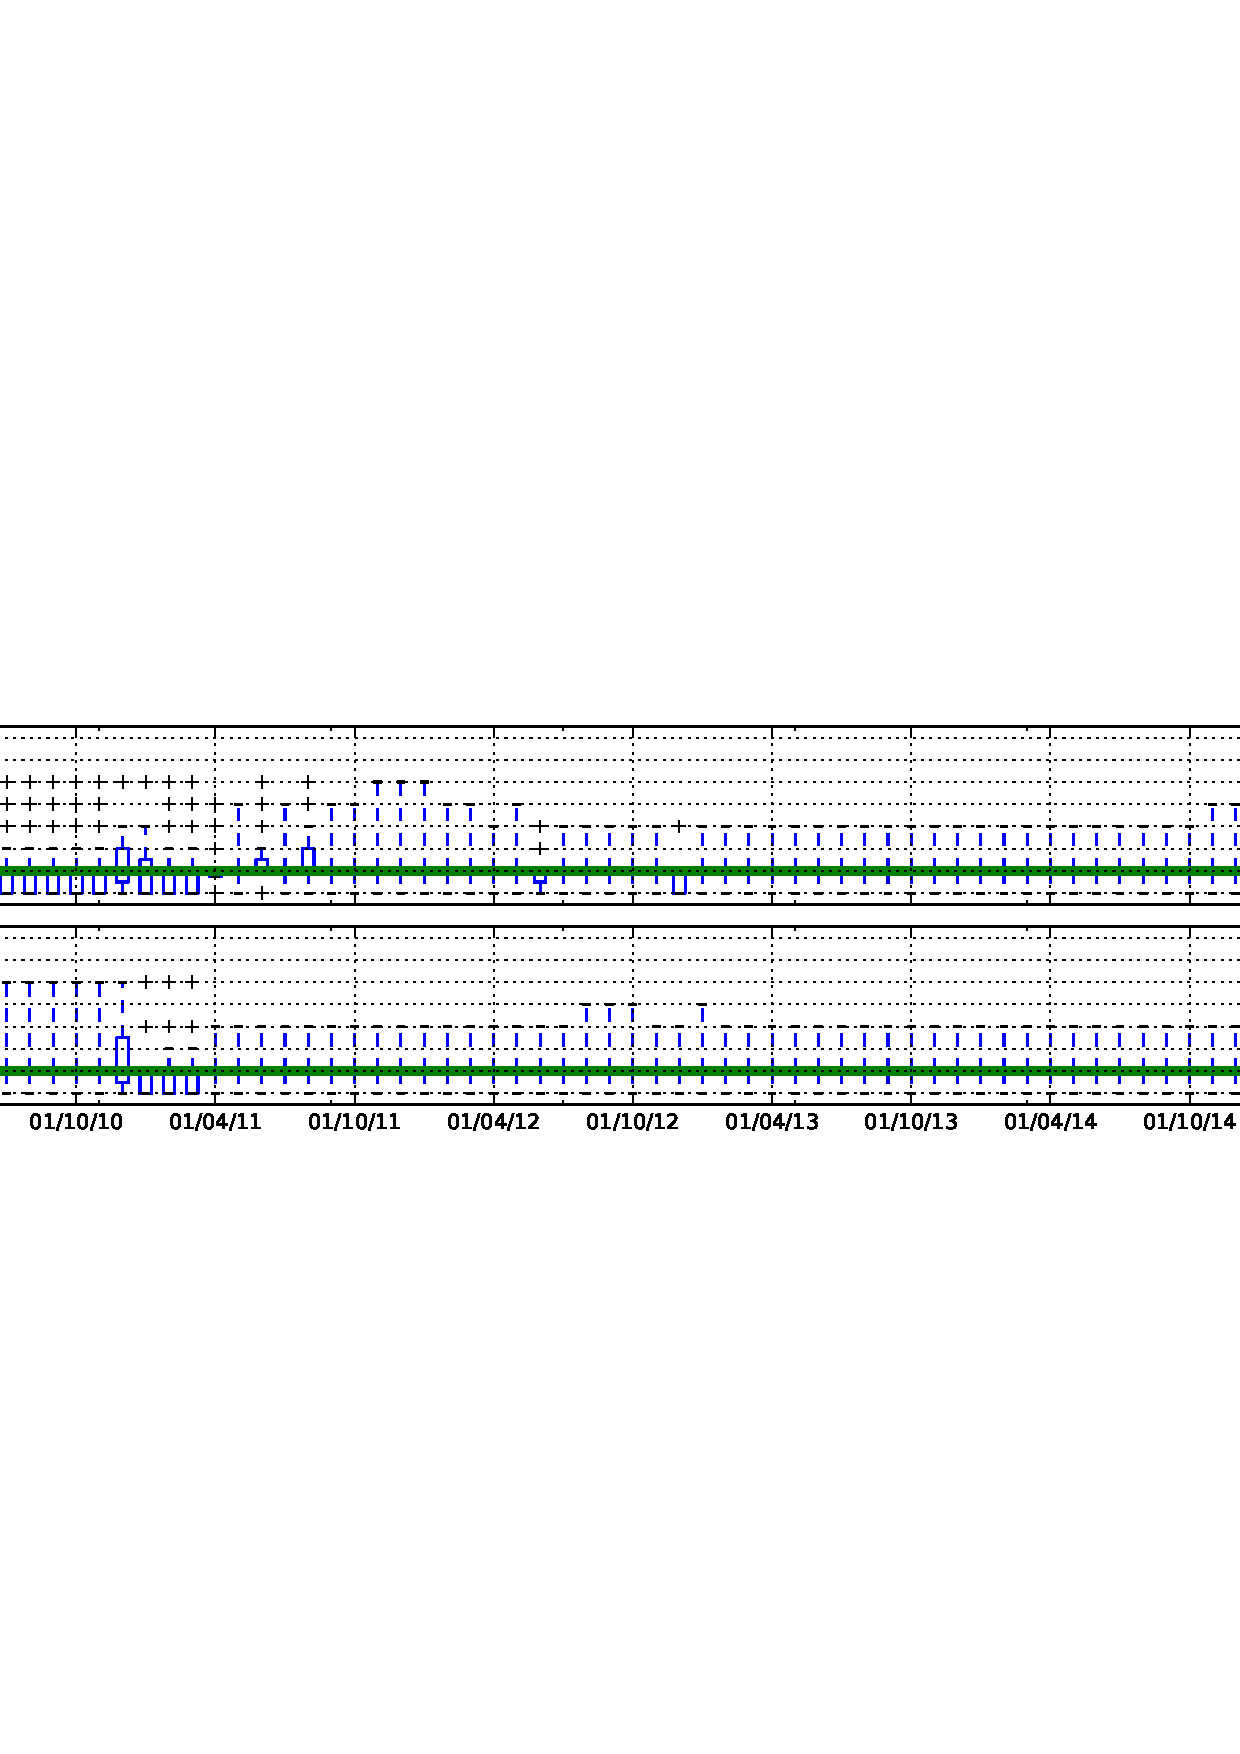
\includegraphics[width=6.0in]{img/path_avg_all_l.png}
			\caption{Path length distribution of all L-Root's VPs}
			\label{fig:path-avg-all-l}
		\end{figure}
		\begin{figure}[htbp]
			\centering
			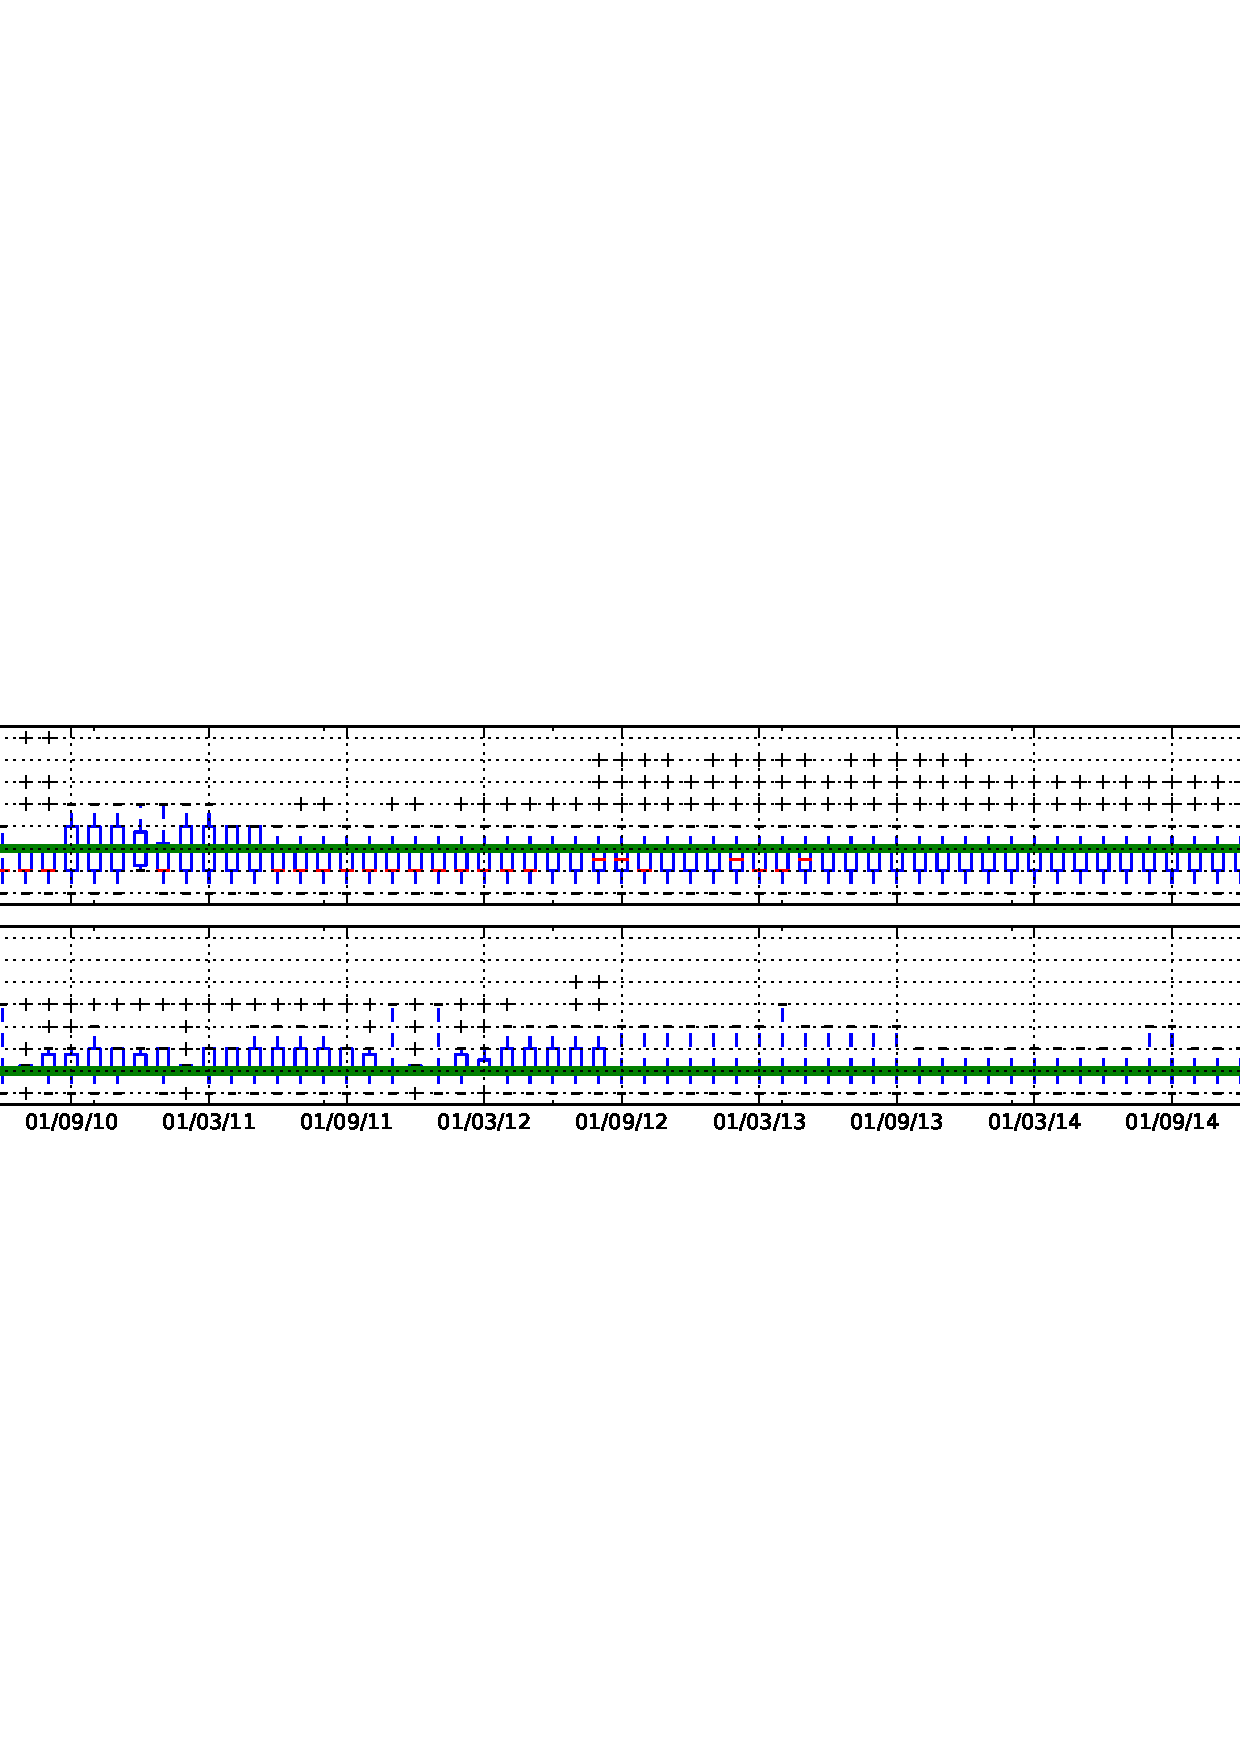
\includegraphics[width=6.0in]{img/path_avg_all_m.png}
			\caption{Path length distribution of all M-Root's VPs}
			\label{fig:path-avg-all-m}
		\end{figure}

	\clearpage		
	\section{Only for VPs with Diverging IPv4/IPv6 Paths}
	\label{app:path-avg:diff-paths}
		\begin{figure}[!htb]
			\centering
			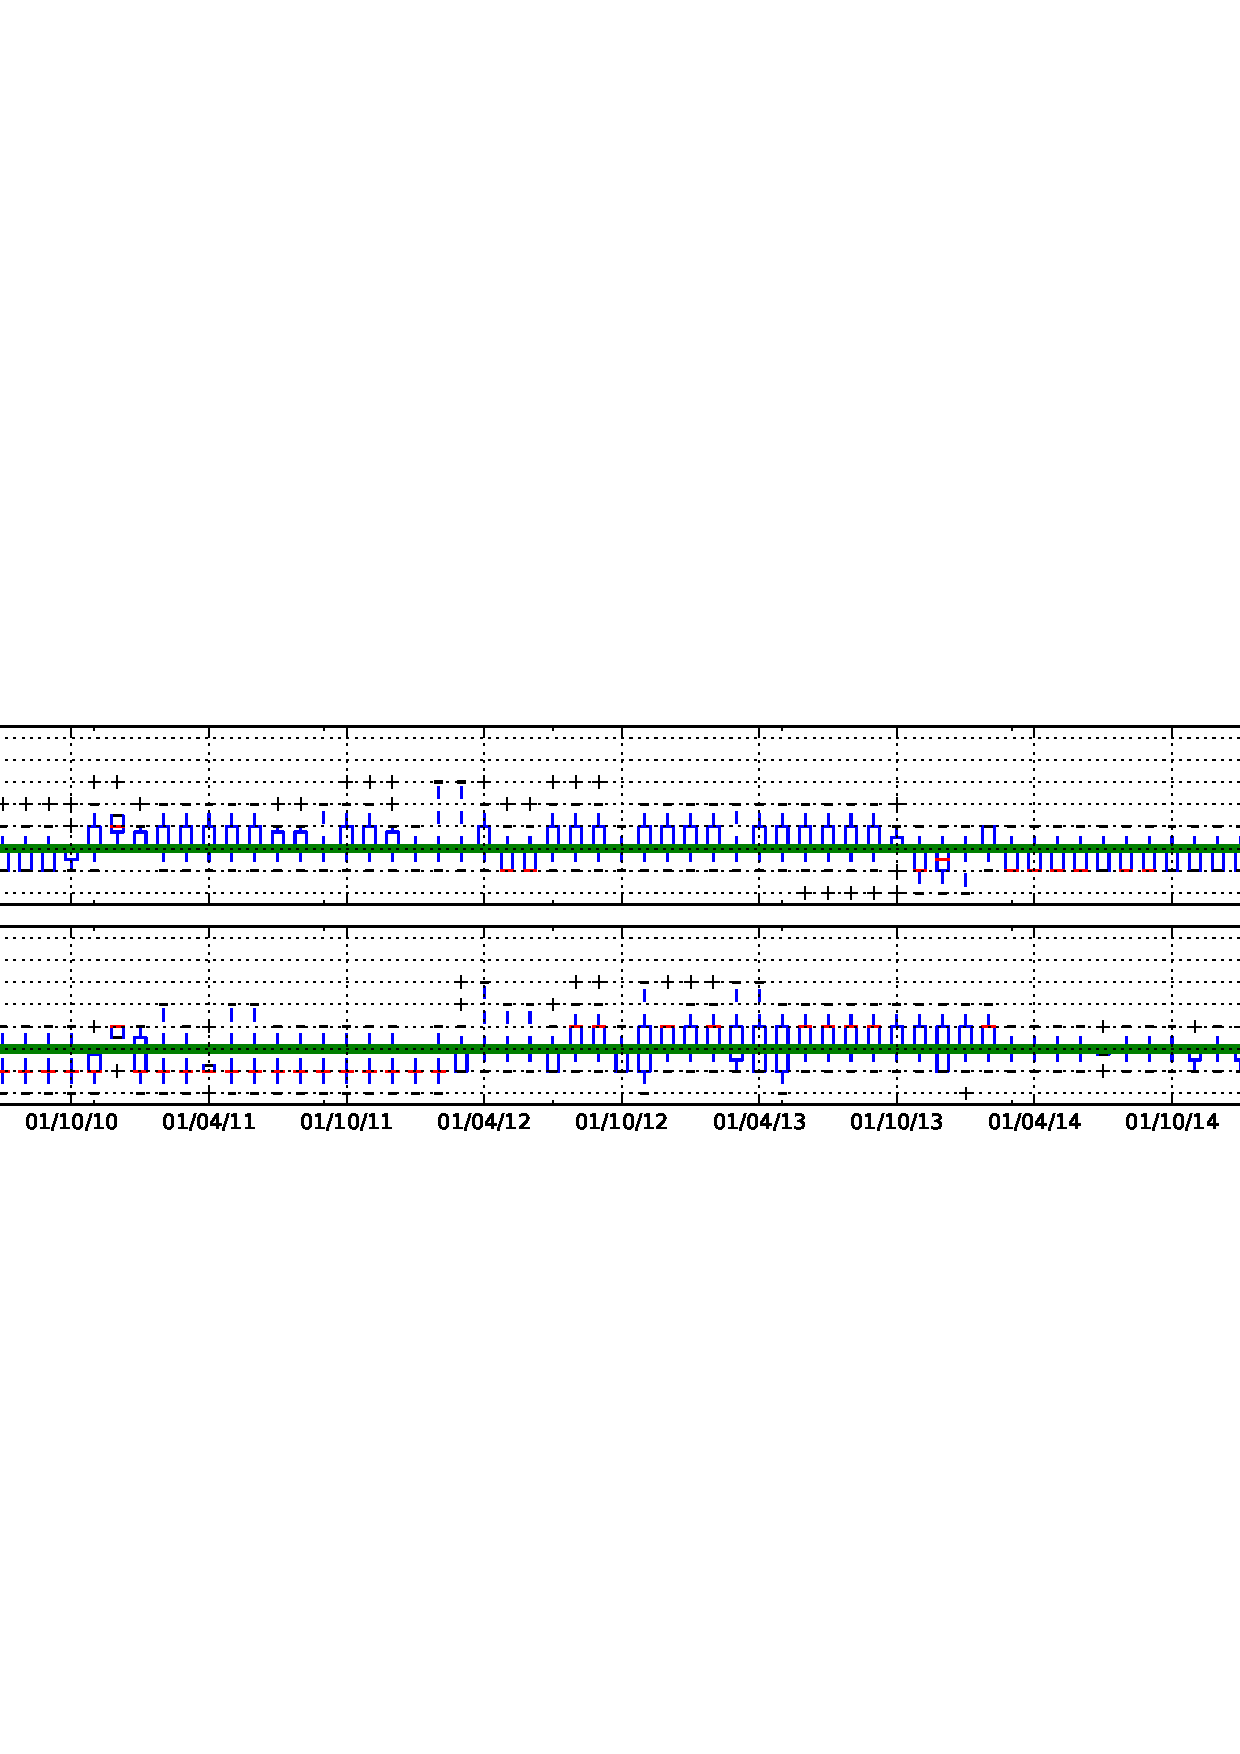
\includegraphics[width=6.0in]{img/path_avg_diff_a.png}
			\caption{Average path length of A-Root peers that have different IPv4/IPv6 paths}
			\label{fig:path-avg-diff-a}
		\end{figure}
		\begin{figure}[!htb]
			\centering
			\includegraphics[width=6.0in]{img/path_avg_diff_c.png}
			\caption{Average path length of C-Root peers that have different IPv4/IPv6 paths}
			\label{fig:path-avg-diff-c}
		\end{figure}
		\begin{figure}[!htb]
			\centering
			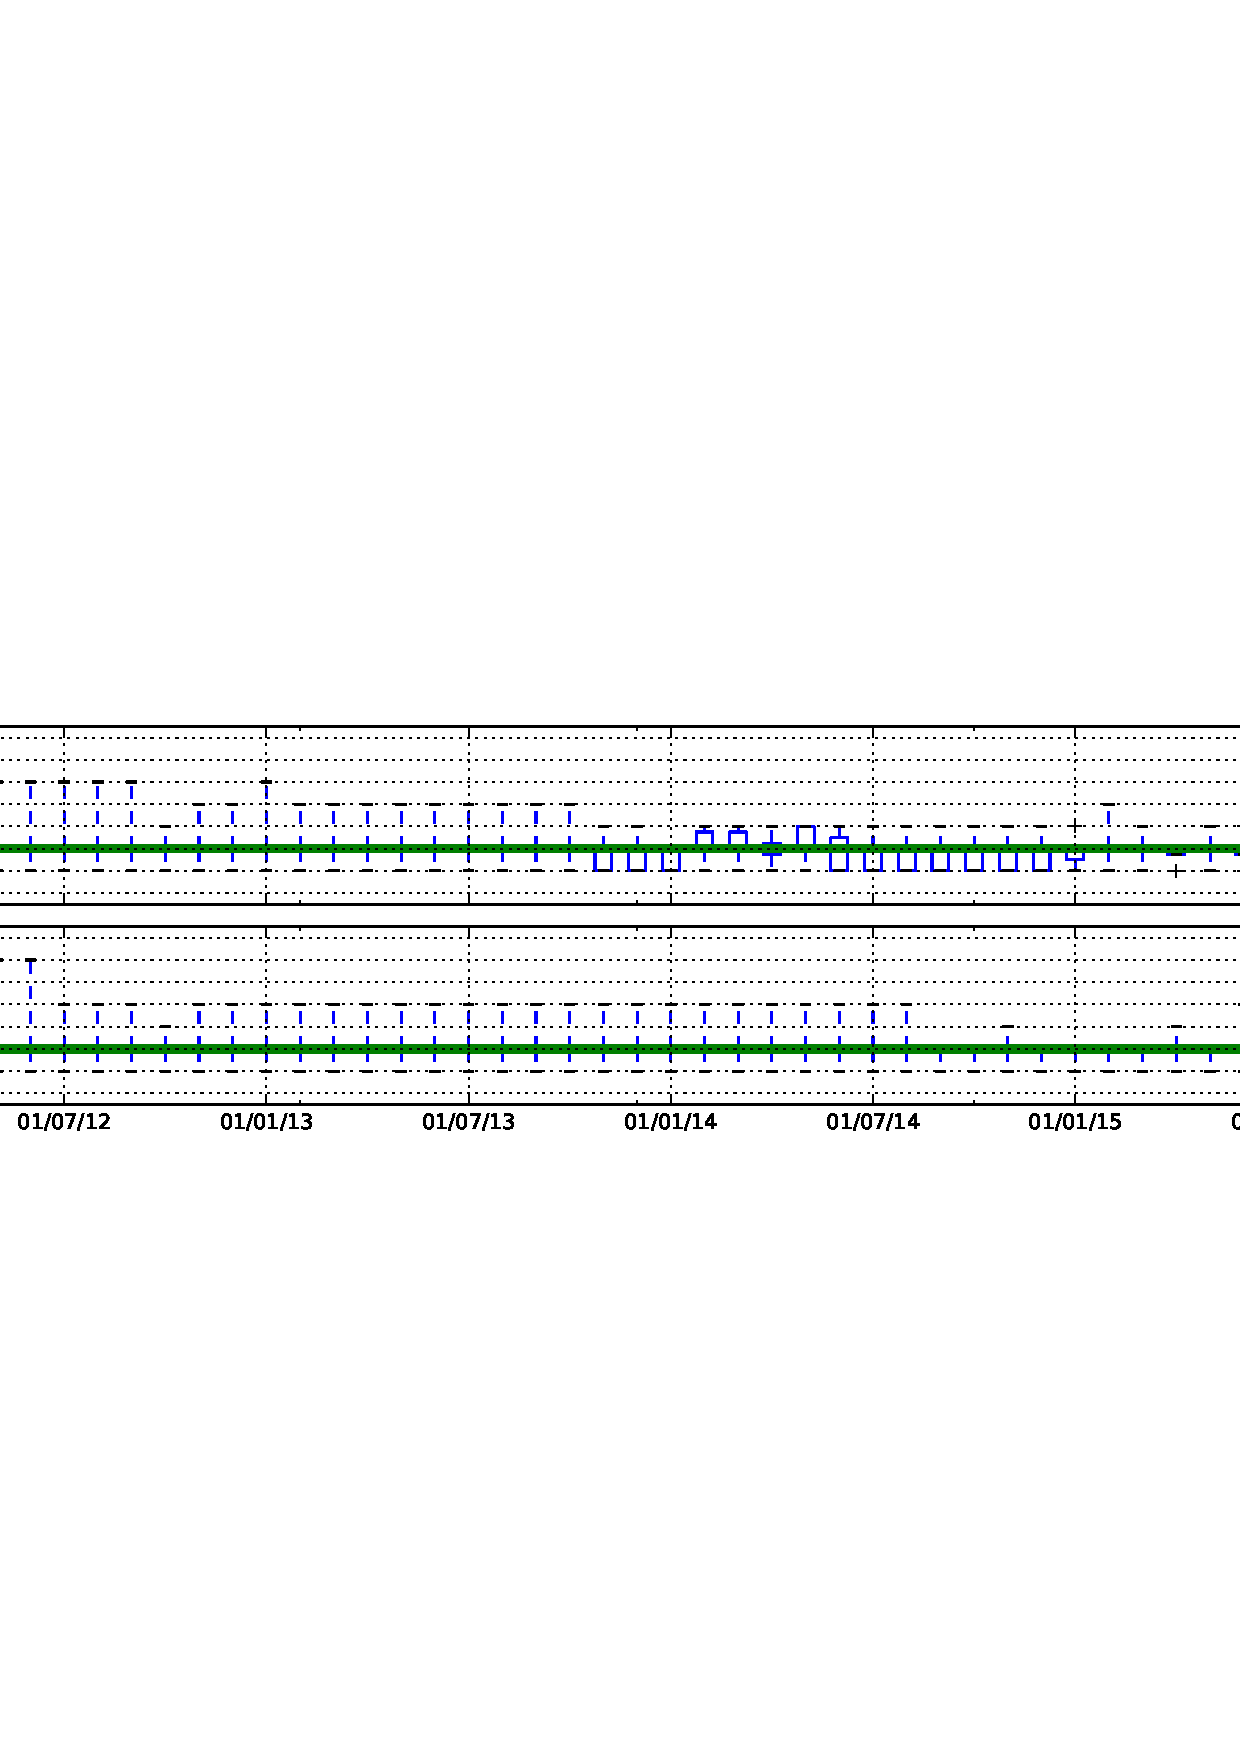
\includegraphics[width=6.0in]{img/path_avg_diff_d.png}
			\caption{Average path length of D-Root peers that have different IPv4/IPv6 paths}
			\label{fig:path-avg-diff-d}
		\end{figure}
		\begin{figure}[!htb]
			\centering
			\includegraphics[width=6.0in]{img/path_avg_diff_f.png}
			\caption{Average path length of F-Root peers that have different IPv4/IPv6 paths}
			\label{fig:path-avg-diff-f}
		\end{figure}
		\begin{figure}[!htb]
			\centering
			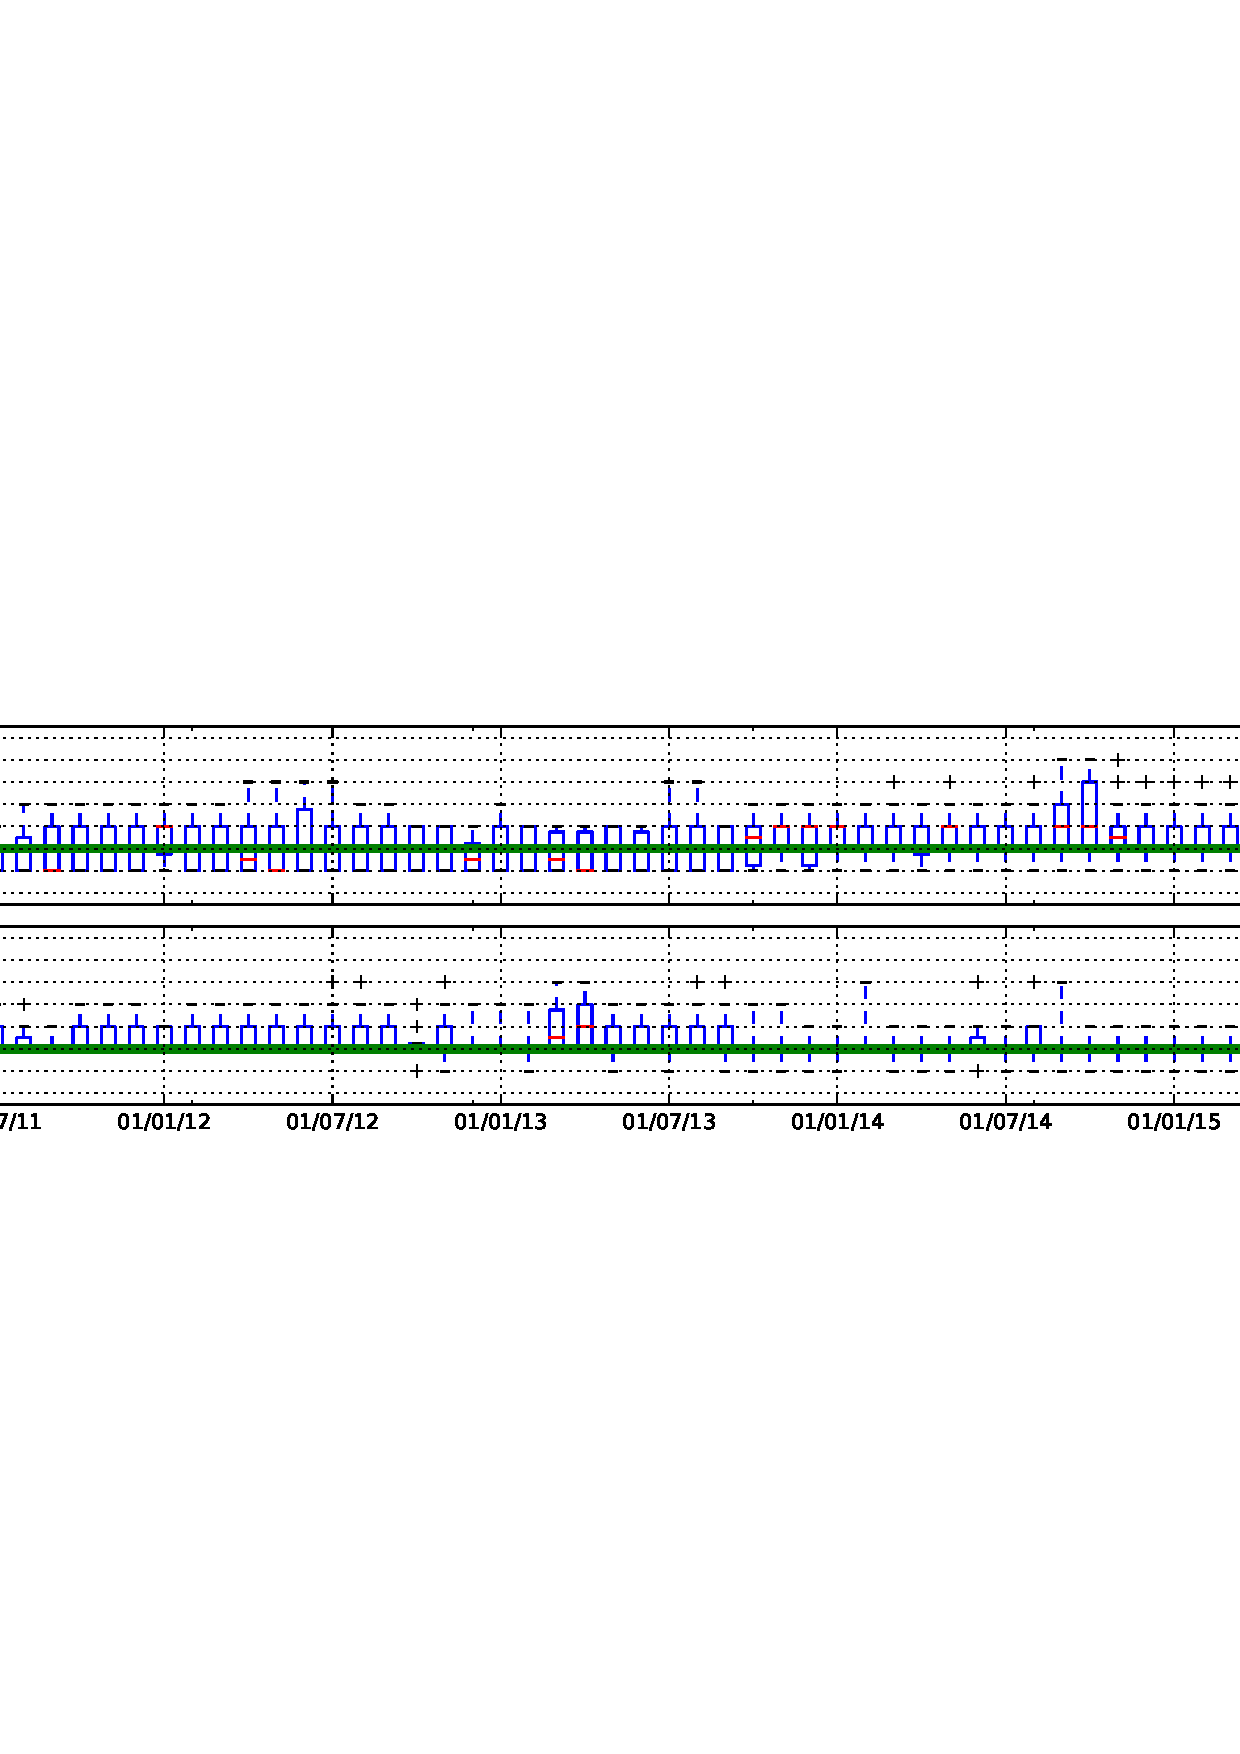
\includegraphics[width=6.0in]{img/path_avg_diff_i.png}
			\caption{Average path length of I-Root peers that have different IPv4/IPv6 paths}
			\label{fig:path-avg-diff-i}
		\end{figure}
		\begin{figure}[!htb]
			\centering
			\includegraphics[width=6.0in]{img/path_avg_diff_j.png}
			\caption{Average path length of J-Root peers that have different IPv4/IPv6 paths}
			\label{fig:path-avg-diff-j}
		\end{figure}
		\begin{figure}[!htb]
			\centering
			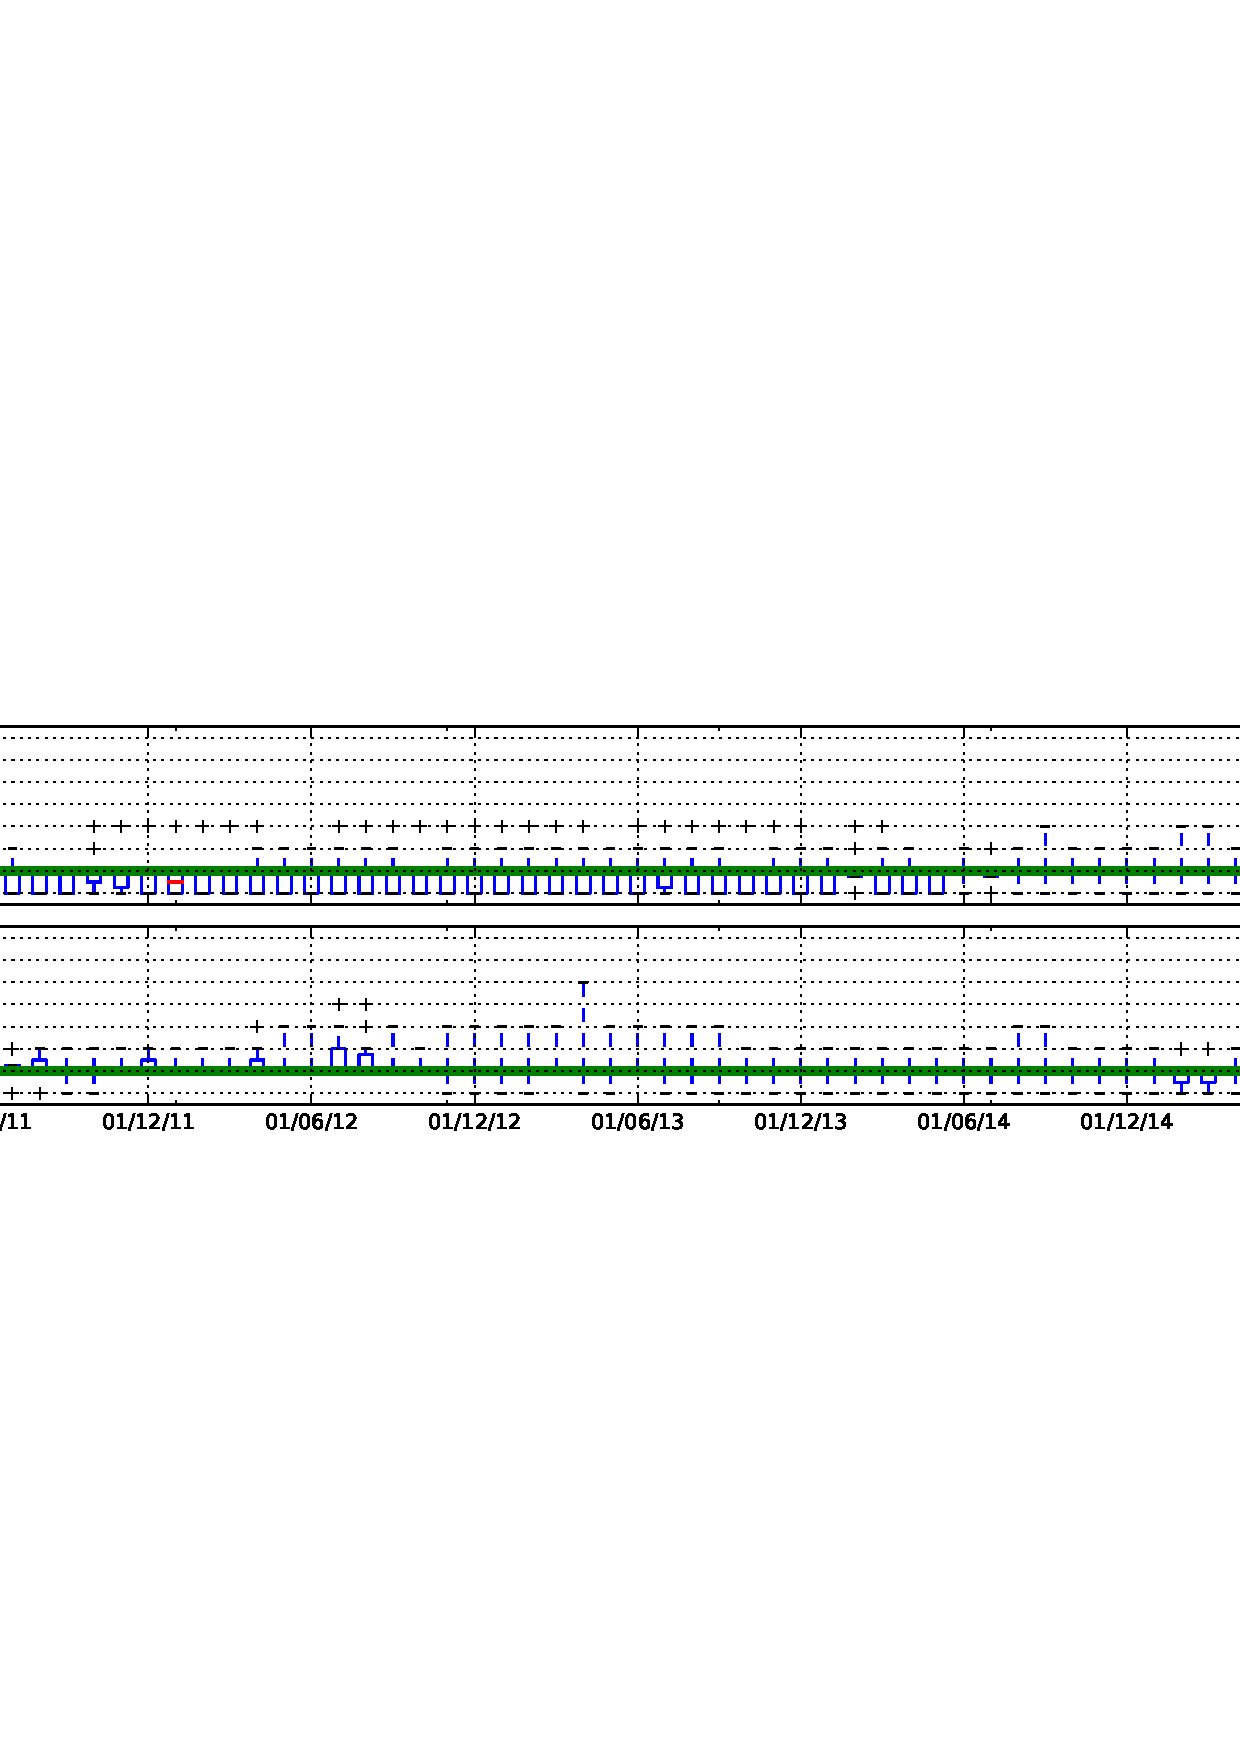
\includegraphics[width=6.0in]{img/path_avg_diff_k.png}
			\caption{Average path length of K-Root peers that have different IPv4/IPv6 paths}
			\label{fig:path-avg-diff-k}
		\end{figure}
		\begin{figure}[!htb]
			\centering
			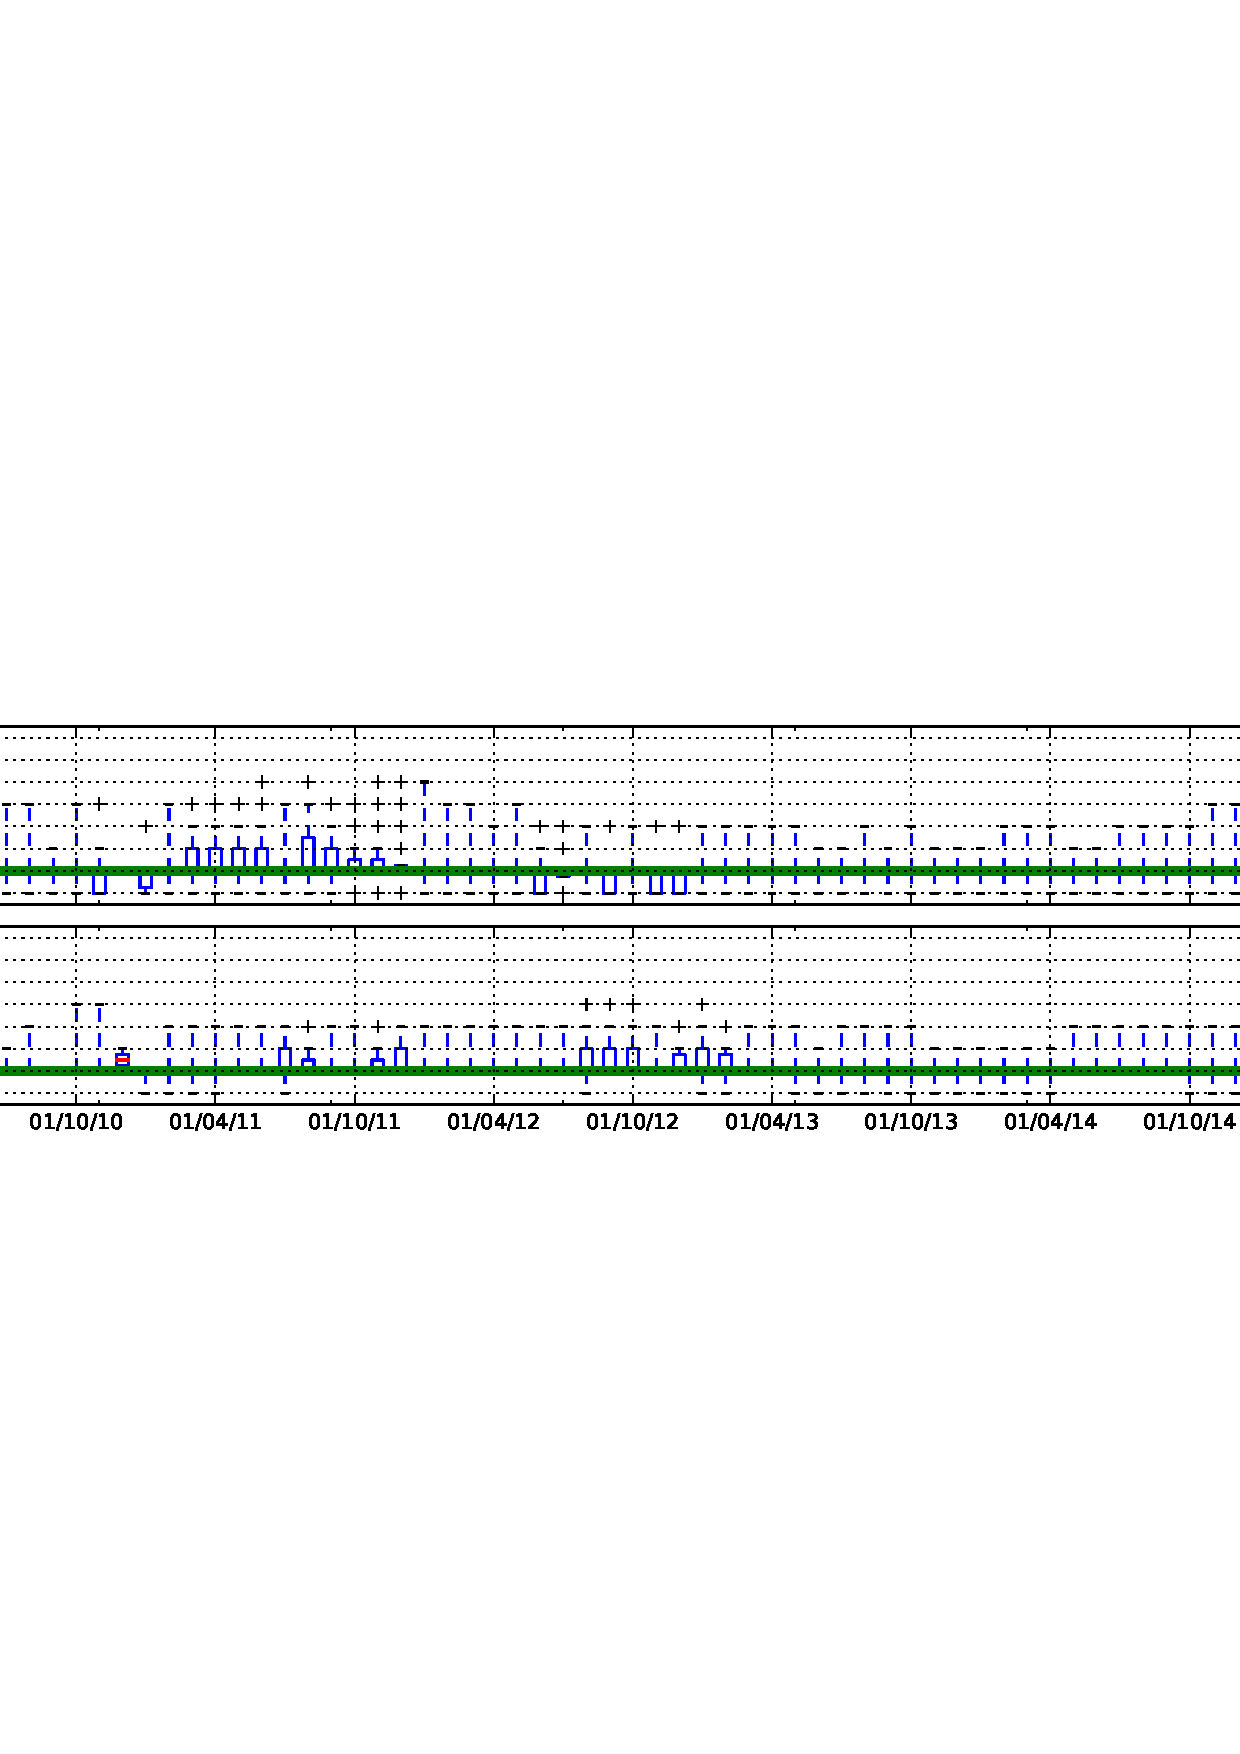
\includegraphics[width=6.0in]{img/path_avg_diff_l.png}
			\caption{Average path length of L-Root peers that have different IPv4/IPv6 paths}
			\label{fig:path-avg-diff-l}
		\end{figure}
		\begin{figure}[!htb]
			\centering
			\includegraphics[width=6.0in]{img/path_avg_diff_m.png}
			\caption{Average path length of M-Root peers that have different IPv4/IPv6 paths}
			\label{fig:path-avg-diff-m}
		\end{figure}	
	
	\chapter{VP Length Degree}
	\label{app:peer-degree-dist}
	The Root Server's diverging VPs 
	
	\begin{figure}[!htb]
		\centering
		\includegraphics[width=6.5in]{img/peer_degree_diff_a.png}
		\caption{VP degree distribution of A-Root}
		\label{fig:app:peer-deg-dist-diff-a}
	\end{figure}
	\begin{figure}[!htb]
		\centering
		\includegraphics[width=6.5in]{img/peer_degree_diff_c.png}
		\caption{VP degree distribution of C-Root}
		\label{fig:app:peer-deg-dist-diff-c}
	\end{figure}
	\begin{figure}[!htb]
		\centering
		\includegraphics[width=6.5in]{img/peer_degree_diff_d.png}
		\caption{VP degree distribution of D-Root}
		\label{fig:app:peer-deg-dist-diff-d}
	\end{figure}
	\begin{figure}
		\centering
		\includegraphics[width=6.5in]{img/peer_degree_diff_f.png}
		\caption{VP degree distribution of F-Root}
		\label{fig:app:peer-deg-dist-diff-f}
	\end{figure}
	\begin{figure}
		\centering
		\includegraphics[width=6.5in]{img/peer_degree_diff_i.png}
		\caption{VP degree distribution of I-Root}
		\label{fig:app:peer-deg-dist-diff-i}
	\end{figure}
	\begin{figure}
		\centering
		\includegraphics[width=6.5in]{img/peer_degree_diff_j.png}
		\caption{VP degree distribution of J-Root}
		\label{fig:app:peer-deg-dist-diff-j}
	\end{figure}
	\begin{figure}
		\centering
		\includegraphics[width=6.5in]{img/peer_degree_diff_k.png}
		\caption{VP degree distribution of K-Root}
		\label{fig:app:peer-deg-dist-diff-k}
	\end{figure}
	\begin{figure}
		\centering
		\includegraphics[width=6.5in]{img/peer_degree_diff_l.png}
		\caption{VP degree distribution of L-Root}
		\label{fig:app:peer-deg-dist-diff-l}
	\end{figure}
	\begin{figure}[!htb]
		\centering
		\includegraphics[width=6.5in]{img/peer_degree_diff_m.png}
		\caption{VP degree distribution of M-Root}
		\label{fig:app:peer-deg-dist-diff-m}
	\end{figure}
	
	
	\chapter{Average Path Length Differences for VPs with Shorter IPv4 Path}
	\label{app:shorter-ipv4}
	\begin{figure}[!htb]
		\centering
		\includegraphics[width=6.0in]{img/shorter-ipv4-a.png}
		\caption{Path length differences for A-Root's VPs with shorter IPv4 path}
		\label{fig:shorter-ipv4-a}
	\end{figure}
	\begin{figure}[!htb]
		\centering
		\includegraphics[width=6.0in]{img/shorter-ipv4-c.png}
		\caption{Path length differences for C-Root's VPs with shorter IPv4 path}
		\label{fig:shorter-ipv4-c}
	\end{figure}
	\begin{figure}[!htb]
		\centering
		\includegraphics[width=6.0in]{img/shorter-ipv4-d.png}
		\caption{Path length differences for D-Root's VPs with shorter IPv4 path}
		\label{fig:shorter-ipv4-d}
	\end{figure}
	\begin{figure}[!htb]
		\centering
		\includegraphics[width=6.0in]{img/shorter-ipv4-f.png}
		\caption{Path length differences for F-Root's VPs with shorter IPv4 path}
		\label{fig:shorter-ipv4-f}
	\end{figure}
	\begin{figure}[!htb]
		\centering
		\includegraphics[width=6.0in]{img/shorter-ipv4-i.png}
		\caption{Path length differences for I-Root's VPs with shorter IPv4 path}
		\label{fig:shorter-ipv4-i}
	\end{figure}
	\begin{figure}[!htb]
		\centering
		\includegraphics[width=6.0in]{img/shorter-ipv4-j.png}
		\caption{Path length differences for J-Root's VPs with shorter IPv4 path}
		\label{fig:shorter-ipv4-j}
	\end{figure}
	\begin{figure}[!htb]
		\centering
		\includegraphics[width=6.0in]{img/shorter-ipv4-k.png}
		\caption{Path length differences for K-Root's VPs with shorter IPv4 path}
		\label{fig:shorter-ipv4-k}
	\end{figure}
	\begin{figure}[!htb]
		\centering
		\includegraphics[width=6.0in]{img/shorter-ipv4-l.png}
		\caption{Path length differences for L-Root's VPs with shorter IPv4 path}
		\label{fig:shorter-ipv4-l}
	\end{figure}
	\begin{figure}[!htb]
		\centering
		\includegraphics[width=6.0in]{img/shorter-ipv4-m.png}
		\caption{Path length differences for M-Root's VPs with shorter IPv4 path}
		\label{fig:shorter-ipv4-m}
	\end{figure}
	
	\chapter{Average Path Length Differences for VPs with Shorter IPv6 Path}
	\label{app:shorter-ipv6}
	\begin{figure}[!htb]
		\centering
		\includegraphics[width=6.0in]{img/shorter-ipv6-a.png}
		\caption{Path length differences for A-Root's VPs with shorter IPv6 path}
		\label{fig:app:shorter-ipv6-a}
	\end{figure}
	\begin{figure}[!htb]
		\centering
		\includegraphics[width=6.0in]{img/shorter-ipv6-c.png}
		\caption{Path length differences for C-Root's VPs with shorter IPv6 path}
		\label{fig:app:shorter-ipv6-c}
	\end{figure}
	\begin{figure}[!htb]
		\centering
		\includegraphics[width=6.0in]{img/shorter-ipv6-d.png}
		\caption{Path length differences for D-Root's VPs with shorter IPv6 path}
		\label{fig:app:shorter-ipv6-d}
	\end{figure}
	\begin{figure}[!htb]
		\centering
		\includegraphics[width=6.0in]{img/shorter-ipv6-f.png}
		\caption{Path length differences for F-Root's VPs with shorter IPv6 path}
		\label{fig:app:shorter-ipv6-f}
	\end{figure}
	\begin{figure}[!htb]
		\centering
		\includegraphics[width=6.0in]{img/shorter-ipv6-i.png}
		\caption{Path length differences for I-Root's VPs with shorter IPv6 path}
		\label{fig:app:shorter-ipv6-i}
	\end{figure}
	\begin{figure}[!htb]
		\centering
		\includegraphics[width=6.0in]{img/shorter-ipv6-j.png}
		\caption{Path length differences for J-Root's VPs with shorter IPv6 path}
		\label{fig:app:shorter-ipv6-j}
	\end{figure}
	\begin{figure}[!htb]
		\centering
		\includegraphics[width=6.0in]{img/shorter-ipv6-k.png}
		\caption{Path length differences for K-Root's VPs with shorter IPv6 path}
		\label{fig:app:shorter-ipv6-k}
	\end{figure}
	\begin{figure}[!htb]
		\centering
		\includegraphics[width=6.0in]{img/shorter-ipv6-l.png}
		\caption{Path length differences for L-Root's VPs with shorter IPv6 path}
		\label{fig:app:shorter-ipv6-l}
	\end{figure}
	\begin{figure}[!htb]
		\centering
		\includegraphics[width=6.0in]{img/shorter-ipv6-m.png}
		\caption{Path length differences for M-Root's VPs with shorter IPv6 path}
		\label{fig:app:shorter-ipv6-m}
	\end{figure}

\iffalse	
	\chapter{Physical Location}
	\label{app:physical-loc}
	\begin{figure}[!htb]
		\centering
		\includegraphics[width=6.0in]{img/coll-ams-ix.png}
		\caption{Peers with different IPv4/IPv6 paths detected by RIS Collector in AMS-IX and NL-IX, Amsterdam}
		\label{fig:coll-ams-ix}
	\end{figure}
	\begin{figure}[!htb]
		\centering
		\includegraphics[width=6.0in]{img/coll-barcelona.png}
		\caption{Peers with different IPv4/IPv6 paths detected by RIS Collector in CATNIX, Barcelona}
		\label{fig:coll-barcelona}
	\end{figure}	
	\begin{figure}[!htb]
		\centering
		\includegraphics[width=6.0in]{img/coll-frankfurt.png}
		\caption{Peers with different IPv4/IPv6 paths detected by RIS Collector in Frankfurt, Germany}
		\label{fig:coll-frankfurt}
	\end{figure}
	\begin{figure}[!htb]
		\centering
		\includegraphics[width=6.0in]{img/coll-geneva.png}
		\caption{Peers with different IPv4/IPv6 paths detected by RIS Collector in CIXP, Geneva}
		\label{fig:coll-geneva}
	\end{figure}	
	\begin{figure}
		\centering
		\includegraphics[width=6.0in]{img/coll-johannesburg.png}
		\caption{Peers with different IPv4/IPv6 paths detected by RIS Collector in NAP Africa JB, Johannesburg}
		\label{fig:coll-johannesburg}
	\end{figure}	
	\begin{figure}[!htb]
		\centering
		\includegraphics[width=6.0in]{img/coll-london.png}
		\caption{Peers with different IPv4/IPv6 paths detected by RIS Collector in LINX, London}
		\label{fig:coll-london}
	\end{figure}
	\begin{figure}[!htb]
		\centering
		\includegraphics[width=6.0in]{img/coll-miami.png}
		\caption{Peers with different IPv4/IPv6 paths detected by RIS Collector in Miami}
		\label{fig:coll-miami}
	\end{figure}	
	\begin{figure}[!htb]
		\centering
		\includegraphics[width=6.0in]{img/coll-milan.png}
		\caption{Peers with different IPv4/IPv6 paths detected by RIS Collector in Milan}
		\label{fig:coll-milan}
	\end{figure}
	\begin{figure}[!htb]
		\centering
		\includegraphics[width=6.0in]{img/coll-moscow.png}
		\caption{Peers with different IPv4/IPv6 paths detected by RIS Collector in Moscow}
		\label{fig:coll-moscow}
	\end{figure}	
	\begin{figure}[!htb]
		\centering
		\includegraphics[width=6.0in]{img/coll-NY.png}
		\caption{Peers with different IPv4/IPv6 paths detected by RIS Collector in New York}
		\label{fig:coll-ny}
	\end{figure}	
	\begin{figure}[!htb]
		\centering
		\includegraphics[width=6.0in]{img/coll-otemachi.png}
		\caption{Peers with different IPv4/IPv6 paths detected by RIS Collector in Otemachi, Tokyo}
		\label{fig:coll-otemachi}
	\end{figure}	
	\begin{figure}[!htb]
		\centering
		\includegraphics[width=6.0in]{img/coll-palo-alto.png}
		\caption{Peers with different IPv4/IPv6 paths detected by RIS Collector in Palo Alto}
		\label{fig:coll-palo-alto}
	\end{figure}	
	\begin{figure}[!htb]
		\centering
		\includegraphics[width=6.0in]{img/coll-paris.png}
		\caption{Peers with different IPv4/IPv6 paths detected by RIS Collector in France IX, Paris}
		\label{fig:coll-paris}
	\end{figure}	
	\begin{figure}[!htb]
		\centering
		\includegraphics[width=6.0in]{img/coll-ripe-ncc.png}
		\caption{Peers with different IPv4/IPv6 paths detected by RIS Collector in RIPE NCC, Amsterdam}
		\label{fig:coll-ripe-ncc}
	\end{figure}	
	\begin{figure}[!htb]
		\centering
		\includegraphics[width=6.0in]{img/coll-sao-paulo.png}
		\caption{Peers with different IPv4/IPv6 paths detected by RIS Collector in Sao Paulo}
		\label{fig:coll-sao-paulo}
	\end{figure}	
	\begin{figure}[!htb]
		\centering
		\includegraphics[width=6.0in]{img/coll-stockholm.png}
		\caption{Peers with different IPv4/IPv6 paths detected by RIS Collector in Stockholm}
		\label{fig:coll-stockholm}
	\end{figure}	
	\begin{figure}[!htb]
		\centering
		\includegraphics[width=6.0in]{img/coll-vienna.png}
		\caption{Peers with different IPv4/IPv6 paths detected by RIS Collector in VIX, Vienna}
		\label{fig:coll-vienna}
	\end{figure}	
	\begin{figure}[!htb]
		\centering
		\includegraphics[width=6.0in]{img/coll-zurich.png}
		\caption{Peers with different IPv4/IPv6 paths detected by RIS Collector in SwissIX, Zurich}
		\label{fig:coll-zurich}
	\end{figure}	
\fi
\end{appendices}

